\documentclass[xcolor=x11names]{beamer}

\usetheme{EIS}

\usepackage{graphicx}
\usepackage{hyperref}
\usepackage{xspace}
\usepackage{attrib}
\usepackage{booktabs}
\usepackage{color}
\usepackage{ragged2e}
\usepackage{multicol}
\usepackage{multirow}
\usepackage[english]{babel}

\usepackage[backend=biber,style=authoryear-comp,natbib=true,isbn=false,url=false,doi=false,eprint=false,dashed=false]{biblatex}
\addbibresource{pmawhorter.bib}

\DeclareCiteCommand{\pcite}{}{\printfield{title} (\printnames{labelname} \printfield{year})}{,}{}

\usepackage{tikz}
\usetikzlibrary{arrows,shapes,backgrounds}

\usepackage{fontspec}
\defaultfontfeatures{Ligatures=TeX}
\newfontfeature{Microtype}{protrusion=default;expansion=default;}
%\setmainfont[Microtype]{Computer Modern Sans}
\usepackage{microtype}
%\setmainfont{Linux Libertine}
%\setsansfont{Linux Biolinum}

\usepackage{array}
\newcolumntype{L}[1]{>{\raggedright\let\newline\\\arraybackslash\hspace{0pt}}m{#1}}
\newcolumntype{C}[1]{>{\centering\let\newline\\\arraybackslash\hspace{0pt}}m{#1}}

\setbeamertemplate{navigation symbols}{}

\newcommand{\quoteshape}{\itshape}
\newcommand{\choicecount}[1]{\fbox{\upshape \sffamily #1}}
\newcommand{\fseed}[1]{\input{fig/framed-seed-#1.tex}}
\newcommand{\work}[1]{\textit{#1}\xspace}
\renewcommand*{\thefootnote}{\ensuremath{\ast}}
\newcommand{\cg}[1]{{\leavevmode\color{gray} #1}}
\newcommand{\pr}[1]{\texttt{#1}}
\newcommand{\prq}[2]{``\texttt{#1}{#2}''}

\newcommand{\ind}{\hspace*{0.8em}}
\newcommand{\svind}{\vspace*{0.3em}}
\newcommand{\vind}{\vspace*{0.5em}}

\def\dunyazad/{\textit{Dunyazad}}
\def\minstrel/{\textit{Minstrel}}
\def\skald/{\textit{Skald}}
\def\problemplanets/{\textit{Problem Planets}}
\def\facade/{\textit{Fa\c{c}ade}}


\title[AI for Understanding Narrative Choices] 
{%
Artificial Intelligence as a Tool for Understanding Narrative Choices%
}

\author[Mawhorter]
{%
  Peter~Mawhorter
}

\institute[UCSC]
{%
  Department of Computer Science \\
  University of California Santa Cruz
}

\date[2016-3-3]
{%
  March 3rd, 2016
}

\begin{document}

\begin{frame}
  \titlepage
\end{frame}

\begin{frame}{Narrative Choices}
\begin{center}
  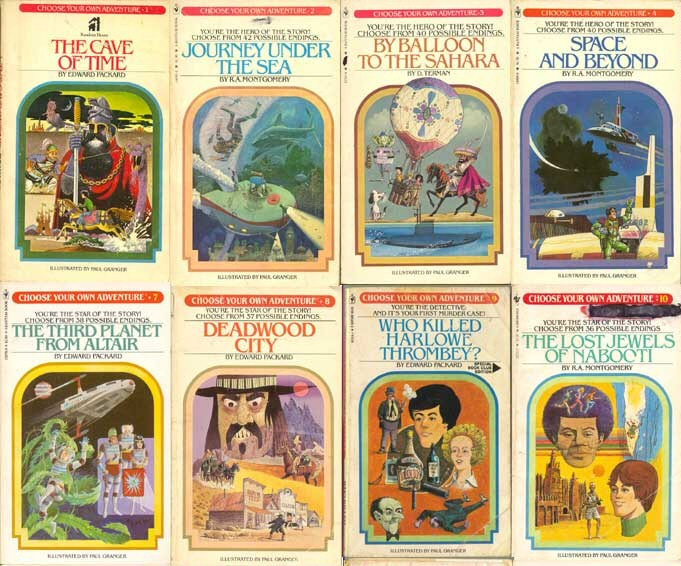
\includegraphics[width=0.8\textwidth]{res/cyoa-covers.jpg}
\end{center}
\end{frame}

\begin{frame}{Narrative Choices}
\begin{center}
  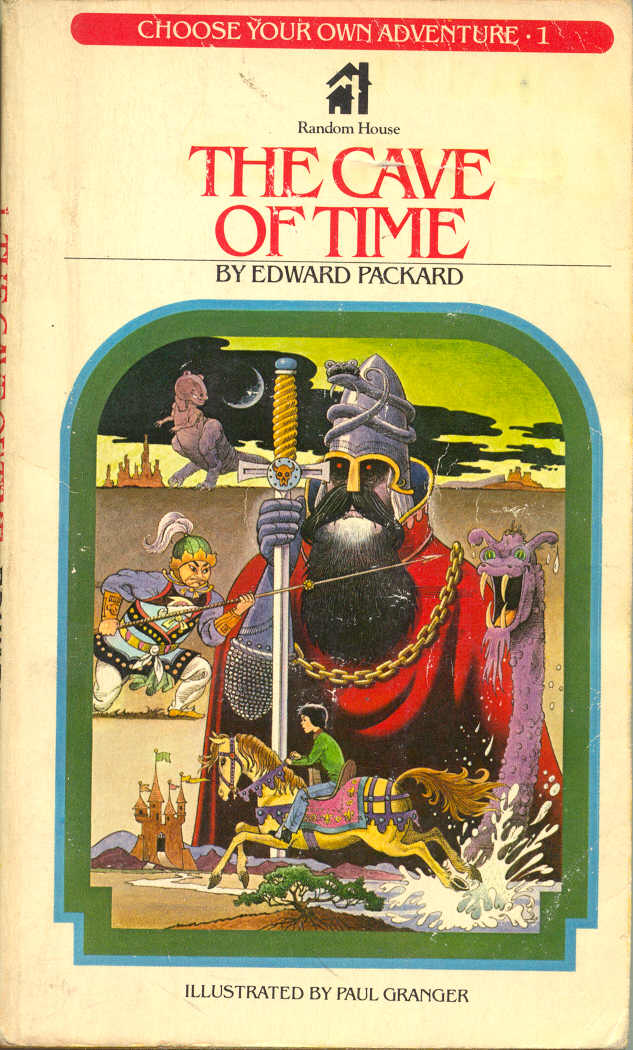
\includegraphics[height=0.8\textheight]{res/cave-of-time-cover.jpg}
  \hspace*{2em}
  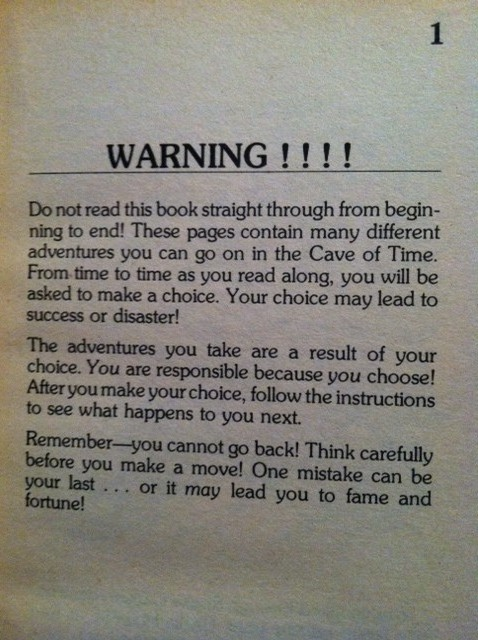
\includegraphics[height=0.8\textheight]{res/cave-of-time-warning.jpg}
\end{center}
\end{frame}

\begin{frame}{Motivation}
\begin{center}
  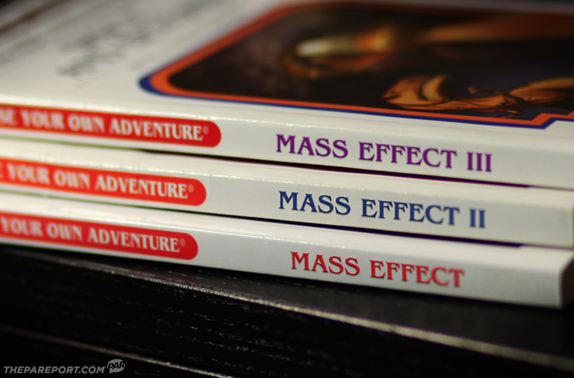
\includegraphics[width=0.95\textwidth]{res/mass-effect-cyoa.jpg}
\end{center}
\end{frame}

\begin{frame}{Motivation: Understanding Popular Culture}
\begin{center}
  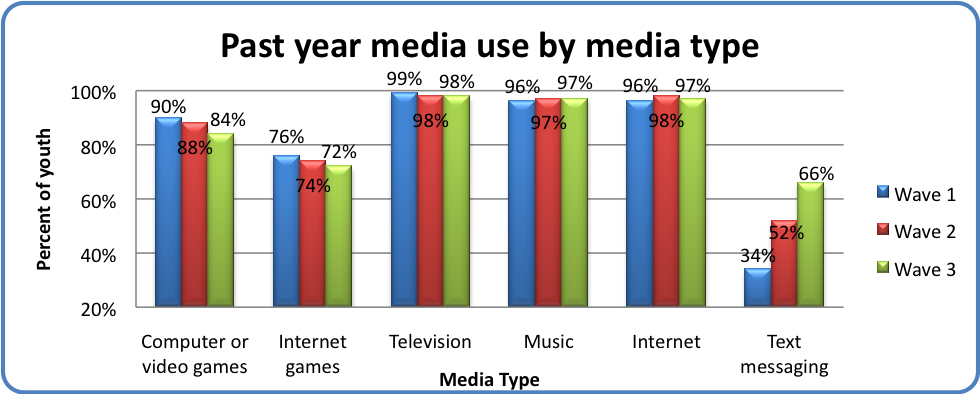
\includegraphics[width=\textwidth]{res/media-use-by-type.png} \\
  \vspace{1em}
  \tiny%
  Graph from the Growing Up With Media longitudinal study 2006--2008; participants were 10--15 years old. \\
  \vspace{1em}
  Published by the Center for Innovative Public Health Research \\
  \vspace{1em}
  \url{https://innovativepublichealth.org/bulletins/growing-up-with-media-media-use-patterns/}
\end{center}
\end{frame}

\begin{frame}{Motivation: Understanding Literature...}
\begin{center}
  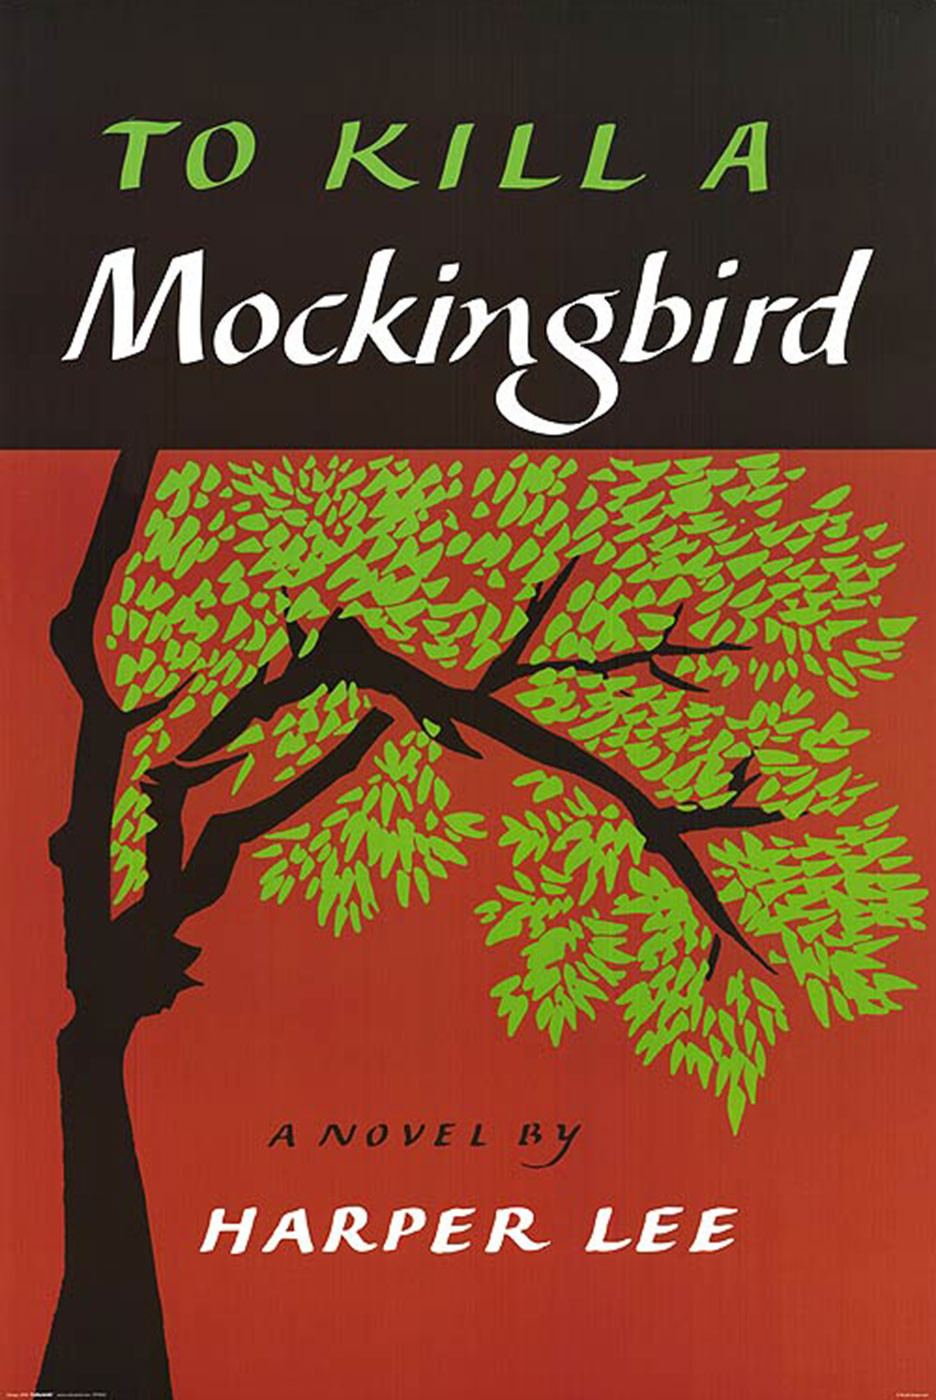
\includegraphics[height=0.8\textheight]{res/to-kill-a-mockingbird-cover.jpg}
  \hspace*{2em}
  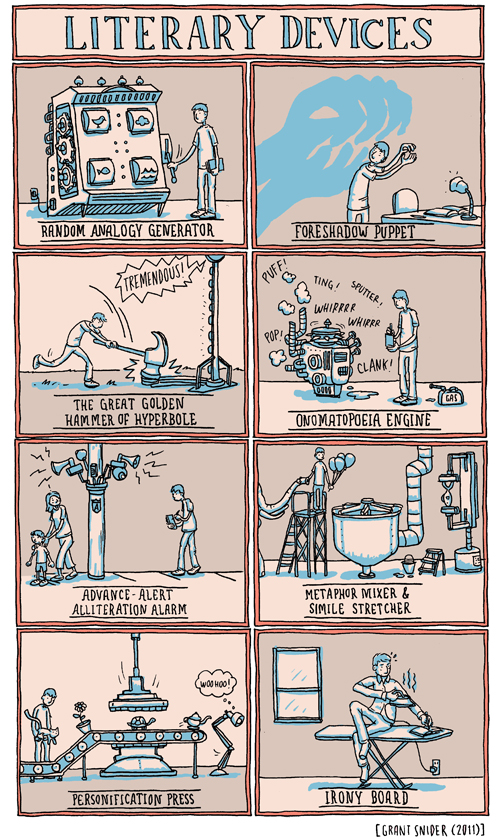
\includegraphics[height=0.8\textheight]{res/literary-devices.jpg}
\end{center}
\end{frame}

\begin{frame}{Motivation: Understanding Games?}
\begin{center}
  
\includegraphics[height=0.45\textheight]{res/journey-title.png}
  \hspace*{1em}
  
\includegraphics[height=0.45\textheight]{res/that-dragon-cancer.png}
  \vspace{1em}
  What can we say about how to understand and interpret these?
\end{center}
\end{frame}

\begin{frame}{Motivation: AI and Society}
\begin{center}
  
\includegraphics[height=0.4\textheight]{res/siri.png}
  \hspace*{1em}
  
\includegraphics[height=0.4\textheight]{res/facebook-ai-research.png}
  \hspace*{1em}
  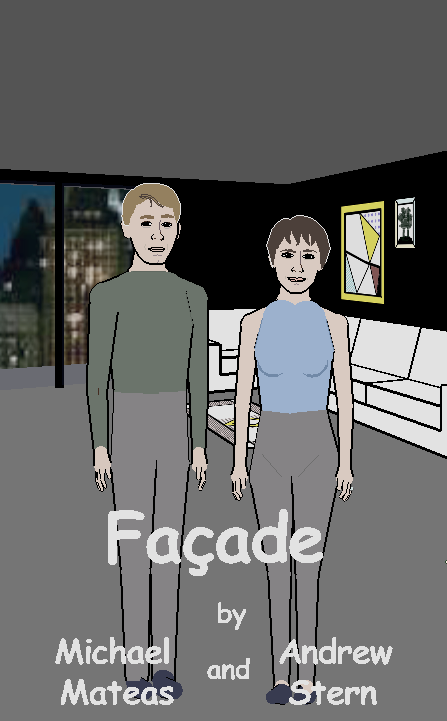
\includegraphics[height=0.4\textheight]{res/facade-title.png} \\
  \vspace{1em}
  If AI is enabling new media and modes of communication, can it also help us understand them?
\end{center}
\end{frame}

%\begin{frame}{My Thesis}
%  \begin{tikzpicture}
%    \node(t)[text width=\textwidth] at (0,0) {%
%      \parbox{0.95\textwidth}{
%  \justifying%
%  \itshape%
%``By reasoning deliberately about choices using a theory of choice poetics, a generative narrative system can construct fixed-form branching narratives that give the player a feeling of agency which persists even when different branches of those narratives are explored.''%
%    }};
%  \end{tikzpicture}
%\end{frame}
%
%\begin{frame}{My Thesis}
%  \vspace*{-0.05ex}%
%  \hspace*{-0.25ex}%
%  \begin{tikzpicture}
%    \node(t)[text width=\textwidth] at (0,0) {%
%      \parbox{0.95\textwidth}{
%  \justifying%
%  \itshape%
%``By reasoning deliberately about choices using a theory of choice poetics, a generative narrative system can construct fixed-form branching narratives that give the player a feeling of agency which persists even when different branches of those narratives are explored.''%
%    }};
%    \draw[color=red,line width=2pt] (t.north west) -- (t.south east);
%    \draw[color=red,line width=2pt] (t.south west) -- (t.north east);
%  \end{tikzpicture}
%\end{frame}

\begin{frame}{My Thesis}
  \justifying
  \itshape
  ``The simultaneous development of a theory for analyzing choice poetics and a system that operationalizes said theory to generate narrative choices provides benefits for both the system and the theory. This novel combination of critical and technical concerns has resulted in an original generative system as well as an analysis framework for understanding choices in terms of player goals.''
\end{frame}

\begin{frame}{My Thesis}
  \justifying
  \itshape
  ``The simultaneous development of a theory for analyzing choice poetics and a system that operationalizes said theory to generate narrative choices provides benefits for both the system and the theory.This \textbf{novel combination of critical and technical concerns} has resulted in an original generative system as well as an analysis framework for understanding choices in terms of player goals.''
\end{frame}

\begin{frame}{My Thesis}
  \justifying
  \itshape
  ``The simultaneous development of a theory for analyzing choice poetics and a system that operationalizes said theory to generate narrative choices provides benefits for both the system and the theory. This novel combination of critical and technical concerns has resulted in \textbf{an original generative system} as well as an analysis framework for understanding choices in terms of player goals.''
\end{frame}

\begin{frame}{My Thesis}
  \justifying
  \itshape
  ``The simultaneous development of a theory for analyzing choice poetics and a system that operationalizes said theory to generate narrative choices provides benefits for both the system and the theory. This novel combination of critical and technical concerns has resulted in an original generative system as well as \textbf{an analysis framework for understanding choices in terms of player goals}.''
\end{frame}

\begin{frame}{Outline}
  \begin{itemize}
    \item Motivation
    \item \textbf{Inspiration: \skald/ and \problemplanets/}
    \item \textbf{Methodology}
    \item \textbf{Related Work}
    \item \textbf{Theory: Choice Poetics}
    \item \textbf{Application: \dunyazad/}
    \item \textbf{Results: Options}
    \item \textbf{Results: Outcomes}
    \item \textbf{Conclusions}
  \end{itemize}
\end{frame}

\begin{frame}{Inspiration}
  \vfill
  \begin{itemize}\addtolength{\itemsep}{0.5\baselineskip}
    \item Brandon Tearse and I build \skald/, a rational reconstruction of Scott Turner's 1993 \minstrel/.
    \item \problemplanets/ attempted to use it for interactive vignettes.
    \item Lessons:
    \begin{itemize}\addtolength{\itemsep}{0.5\baselineskip}
      \vspace{0.5\baselineskip}
      \item Focus on the consistency rules---raw material can be random.
      \item Come up with principles for placement and structure of choices.
    \end{itemize}
  \end{itemize}
  \vfill
  \centering
  \tiny
  \pcite{Turner1993} \\
  \pcite{Tearse2014}
\end{frame}

\begin{frame}{Outline}
  \begin{itemize}
    \item Motivation
    \item Inspiration: \skald/ and \problemplanets/
    \item \textbf{Methodology}
    \item \textbf{Related Work}
    \item \textbf{Theory: Choice Poetics}
    \item \textbf{Application: \dunyazad/}
    \item \textbf{Results: Options}
    \item \textbf{Results: Outcomes}
    \item \textbf{Conclusions}
  \end{itemize}
\end{frame}

\begin{frame}{Research Approach}
  \begin{itemize}\addtolength{\itemsep}{0.5\baselineskip}
    \item To intentionally construct choices requires goals and strategies:%
    \begin{itemize}\addtolength{\itemsep}{0.5\baselineskip}
      \vspace{0.5\baselineskip}
      \item Goals: poetic effects (e.g., obviousness).
      \item Strategies: a theory of choice poetics.
    \end{itemize}
    \item Existing theories are fragmented and focused elsewhere.
    \begin{itemize}\addtolength{\itemsep}{0.5\baselineskip}
      \vspace{0.5\baselineskip}
      \item Link poetics.
      \item Decision affect theory.
      \item Craft advice.
    \end{itemize}
  \end{itemize}
\end{frame}

\begin{frame}{Choice Poetics}
  \vfill
  \begin{itemize}\addtolength{\itemsep}{0.5\baselineskip}
      \item How do certain \textbf{choice structures} promote particular \textbf{poetic effects}?
    \begin{itemize}\addtolength{\itemsep}{0.5\baselineskip}
      \vspace{0.5\baselineskip}
      \item What is a \textbf{choice structure}?
      \item What \textbf{poetic effects} are possible?
      \item How do \textbf{player perspectives} affect the perception of choices?
    \end{itemize}
  \end{itemize}
  \vfill
  \centering
  \tiny
  \pcite{Mawhorter2014}
\end{frame}

\begin{frame}{Choice Poetics}
  \hspace*{-2em}%
  \begin{tabular}{p{1em} p{\textwidth}}
  \vspace{2.25em}
  
\includegraphics[width=3.5em]{res/stacked-books.jpg} \newline
  \vspace{2em}
  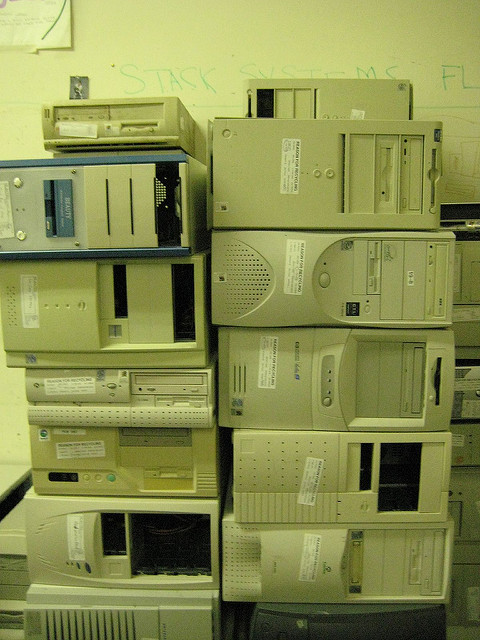
\includegraphics[width=3.5em]{res/stacked-computers.jpg}
  &
  \begin{itemize}\addtolength{\itemsep}{0.5\baselineskip}
      \item Classic approach: Carefully study existing narrative choices.
    \begin{itemize}\addtolength{\itemsep}{0.5\baselineskip}
      \vspace{0.5\baselineskip}
      \item Observe specific constructions and try to generalize them.
      \item Contrast works to show links between structure and poetics.
    \end{itemize}
    \item AI-based approach: Formalize intuitions and experiment.
    \begin{itemize}\addtolength{\itemsep}{0.5\baselineskip}
      \vspace{0.5\baselineskip}
      \item Express observed properties/relationships as logical rules.
      \item Generate choices which obey those rules.
      \item Add rules to correct/refine results.
      \item Translate added rules back into theoretical statements.
    \end{itemize}
    \pause
  \item \emph{Both approaches can inform each other.}
  \end{itemize}
  \end{tabular}
\end{frame}

\begin{frame}{Outline}
  \begin{itemize}
    \item Motivation
    \item Inspiration: \skald/ and \problemplanets/
    \item Methodology
    \item \textbf{Related Work}
    \item \textbf{Theory: Choice Poetics}
    \item \textbf{Application: \dunyazad/}
    \item \textbf{Results: Options}
    \item \textbf{Results: Outcomes}
    \item \textbf{Conclusions}
  \end{itemize}
\end{frame}

\begin{frame}{Related Work}
  \begin{itemize}\addtolength{\itemsep}{0.5\baselineskip}
    \item Criticism and Analysis
    \item Psychology and Cognitive Science
    \item Generative Systems
  \end{itemize}
\end{frame}

\begin{frame}{Criticism and Analysis}
  \begin{itemize}\addtolength{\itemsep}{0.5\baselineskip}
    \item Criticism and Analysis
    \begin{itemize}\addtolength{\itemsep}{0.5\baselineskip}
      \vspace{0.5\baselineskip}
      \item Formalist literary theory \\ \vspace{0.3\baselineskip}
        \tiny
        \pcite{Propp1971} \\
        \pcite{Barthes1975} \\
        \pcite{Greimas1988}

      \item \small Theories of Interactive Media \\ \vspace{0.3\baselineskip}
        \tiny
        \pcite{Murray1997} \\
        \pcite{Tosca1999} \\
        \pcite{WardripFruin2009} \\
        \pcite{Treanor2013} \\
        \pcite{Mitchell2012}

      \item \small Craft Advice \\ \vspace{0.3\baselineskip}
        \tiny
        \pcite{Laws2001} \\
        \pcite{ChoiceOfGamesChoiceRules}
    \end{itemize}
  \end{itemize}
\end{frame}

\begin{frame}{Psychology and Cognitive Science}
  \begin{itemize}\addtolength{\itemsep}{0.5\baselineskip}
    \item Psychology and Cognitive Science
    \begin{itemize}\addtolength{\itemsep}{0.5\baselineskip}
      \vspace{0.5\baselineskip}
      \item Specific effects (e.g., suspense; identification)\\ \vspace{0.3\baselineskip}
        \tiny
        \pcite{Gerrig1994} \\
        \pcite{Oatley1995}

      \item \small Science-informed criticism  \\ \vspace{0.3\baselineskip}
        \tiny
        \pcite{Palmer2004} \\
        \pcite{Zunshine2006}

      \item \small The psychology of decision-making \\ \vspace{0.3\baselineskip}
        \tiny
        \pcite{Tversky1993} \\
        \pcite{Mellers1999} \\
        \pcite{Schwartz2002}
    \end{itemize}
  \end{itemize}
\end{frame}

%\begin{frame}{Decision Affect Theory}
%\end{frame}

\begin{frame}{Generative Systems}
  \begin{itemize}\addtolength{\itemsep}{0.5\baselineskip}
    \item Generative Systems
    \begin{itemize}\addtolength{\itemsep}{0.5\baselineskip}
      \vspace{0.5\baselineskip}
      \item Effect-focused systems \\ \vspace{0.3\baselineskip}
        \tiny
        \pcite{Cheong2006} \\
        \pcite{Bae2008} \\
        \pcite{Ware2014}

      \item \small Interactive narrative systems \\ \vspace{0.3\baselineskip}
        \tiny
        \pcite{Szilas2003} \\
        \pcite{Barber2007a} \\
        \pcite{Yu2013}

      \item \small Player modelling \\ \vspace{0.3\baselineskip}
        \tiny
        \pcite{Mott2006} \\
        \pcite{Thue2008}
    \end{itemize}
  \end{itemize}
\end{frame}

%\begin{frame}{Dilemma-Based Interactive Fiction}
%\end{frame}

%\begin{frame}{Collaborative Filtering}
%\end{frame}

\begin{frame}{Outline}
  \begin{itemize}
    \item Motivation
    \item Inspiration: \skald/ and \problemplanets/
    \item Methodology
    \item Related Work
    \item \textbf{Theory: Choice Poetics}
    \item \textbf{Application: \dunyazad/}
    \item \textbf{Results: Options}
    \item \textbf{Results: Outcomes}
    \item \textbf{Conclusions}
  \end{itemize}
\end{frame}

\begin{frame}{Poetic Effects}
  \vfill
  \centering
  \begin{quote}
  \itshape
  The trees are in their autumn beauty, \\
  The woodland paths are dry, \\
  Under the October twilight the water \\
  Mirrors a still sky;
\end{quote}
\raggedleft
  -from \work{The Wild Swans At Coole} by William Butler Yeats \\
  \vfill
  \raggedright
  Broadly, \textbf{poetics} is the study of how literary techniques provoke audience reactions (the complement of hermeneutics).
\end{frame}

\begin{frame}{Poetic Effects}
  \centering
  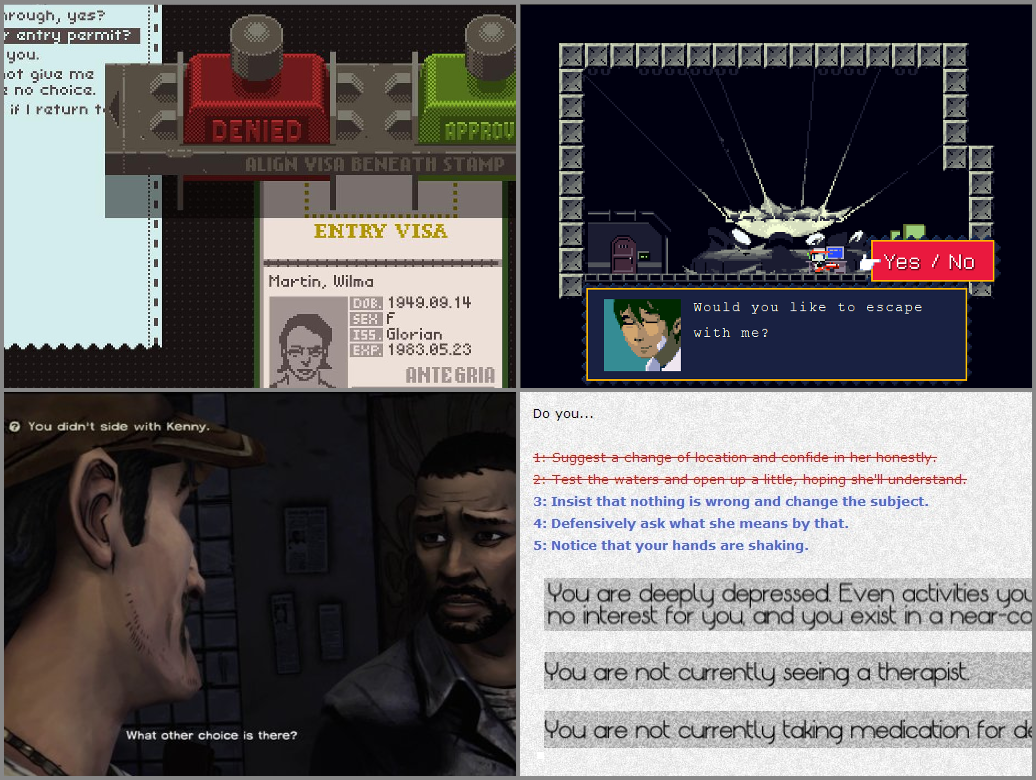
\includegraphics[height=0.8\textheight]{res/four-choices.png} \\
  \vspace{0.5ex}
  \textbf{Choice poetics} applies this to choices in narrative contexts.
\end{frame}

\begin{frame}{Choice Poetics}
  \vfill
  \begin{itemize}\addtolength{\itemsep}{0.5\baselineskip}
      \item How do certain \textbf{choice structures} promote particular \textbf{poetic effects}?
    \begin{itemize}\addtolength{\itemsep}{0.5\baselineskip}
      \vspace{0.5\baselineskip}
      \item What is a \textbf{choice structure}?
      \item What \textbf{poetic effects} are possible?
      \item How do \textbf{player perspectives} affect the perception of choices?
    \end{itemize}
  \end{itemize}
  \vfill
  \centering
  \tiny
  \pcite{Mawhorter2014}
\end{frame}

\begin{frame}{Choice Poetics}
  \begin{itemize}\addtolength{\itemsep}{0.5\baselineskip}
      \item \textbf{What is a choice?}
      \item \textbf{Modes of engagement}
      \item \textbf{Poetic effects}
      \item \textbf{Goal-based choice analysis}
  \end{itemize}
\end{frame}

\begin{frame}{Choice Structure}
  \begin{itemize}\addtolength{\itemsep}{0.5\baselineskip}
    \item Explicit, discrete choices:
    \begin{itemize}\addtolength{\itemsep}{0.5\baselineskip}
      \vspace{0.5\baselineskip}
      \item Framing
      \item Options
      \item Outcomes
      \begin{itemize}\addtolength{\itemsep}{0.5\baselineskip}
        \vspace{0.5\baselineskip}
        \item Outcome components
      \end{itemize}
    \end{itemize}
  \end{itemize}
\end{frame}

\begin{frame}{Choice Structure}
  \vspace{1ex}
  \begin{tabular}{p{0.15\textwidth} l}
    \vspace*{-0.5ex}
    \vtop{
      \null
      \hbox{\hspace{2em} framing $\left\{\rule{0pt}{14.5ex}\right.$}
      \hbox{\rule{0pt}{0.5ex}}
      \hbox{\hspace{2.2em} options $\left\{\rule{0pt}{3.5ex}\right.$\hspace*{-2ex}}
    }
    &
  \vtop{\null\hbox{%
  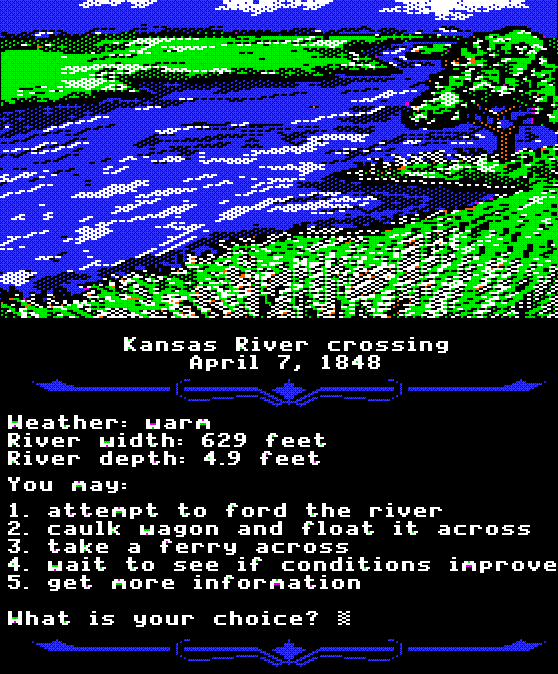
\includegraphics[width=0.5\textwidth]{res/oregon-trail-kansas-river-choice.png}
  }}
  \end{tabular}
\end{frame}

\begin{frame}{Choice Structure}
  \centering
  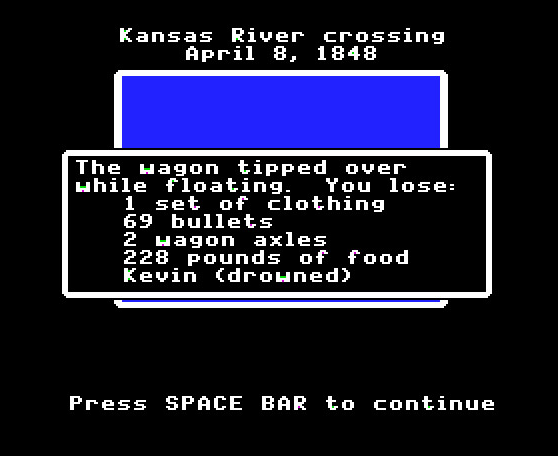
\includegraphics[width=0.5\textwidth]{res/oregon-trail-kansas-river-outcome.png} \\ \vspace{1ex}
  One possible outcome (with five apparent components).
\end{frame}

\begin{frame}{Choice Poetics}
  \begin{itemize}\addtolength{\itemsep}{0.5\baselineskip}
      \item What is a choice?
      \item \textbf{Modes of engagement}
      \item \textbf{Poetic effects}
      \item \textbf{Goal-based choice analysis}
  \end{itemize}
\end{frame}

\begin{frame}{Modes of Engagement}
  \hbox{
    \vtop{
      \null%
      \hbox{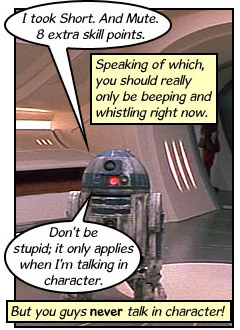
\includegraphics[width=0.28\textwidth]{res/r2d2minmax.jpg}}
    }
    \vtop{
      \null%
      \parbox{0.6\textwidth}{
      \begin{itemize}\addtolength{\itemsep}{0.5\baselineskip}
          \item \textbf{Reasons to play} are distinct from \textbf{reasons to decide}.
          \item Player goals determine how players evaluate options.
          \item \textbf{Modes of engagement} are frameworks for player goals.
      \end{itemize}
      }
    }
  }
\vfill
\tiny
\centering
\pcite{Yee2006} \\
\pcite{Kallio2011} \\
\pcite{Hamari2014}
\end{frame}

\begin{frame}{Modes of Engagement}
\vfill
\centering
\renewcommand*{\arraystretch}{1.5}
\scriptsize
\begin{tabular}{p{6em}p{12em}p{13em}}
\toprule
\textbf{Mode} & \textbf{Decision Process} & \textbf{Example} \\
\midrule
\textbf{Avatar Play} & Decide as if you were in the character's situation. & When picking a pet, pick the cat because you like cats. \\
\textbf{Role Play} & Decide in order to act out a persona. & Choose the wizard character class because you want to play a shy, bookish person. \\
\textbf{Power Play} & Choose options that advance game metrics like score, beating other players, or quick completion. & Sacrifice an ally to obtain a powerful item because it helps you beat the game more quickly. \\
\textbf{Exploratory Play} & Choose options to see what will happen. & Turn away from the path of your quest to explore the world. \\
\textbf{Social Play} & In a multiplayer situation, choose options because of social considerations. & Turn down a high-level quest in order to accompany your friend on a lower-level quest. \\
\bottomrule
\end{tabular} \\ \vspace{1ex}
\ldots and more, for example \textbf{analytical play} and \textbf{critical play}.
\end{frame}

\begin{frame}{Choice Poetics}
  \begin{itemize}\addtolength{\itemsep}{0.5\baselineskip}
      \item What is a choice?
      \item Modes of engagement
      \item \textbf{Poetic effects}
      \item \textbf{Goal-based choice analysis}
  \end{itemize}
\end{frame}

\begin{frame}{Poetic Effects}
  \centering
  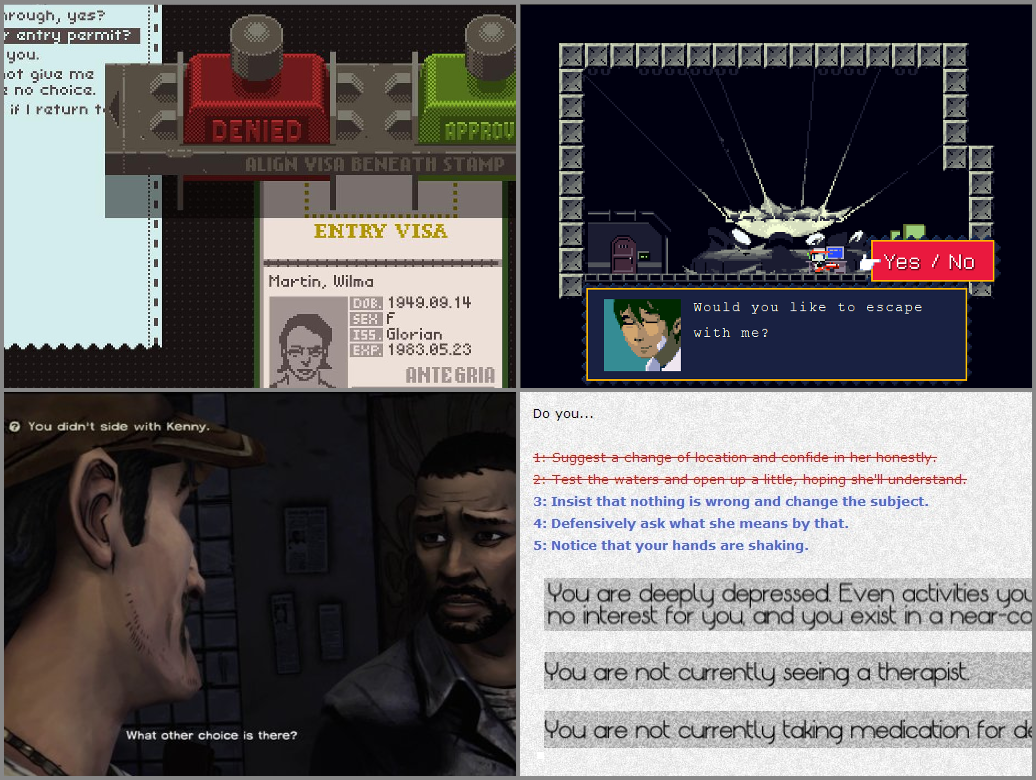
\includegraphics[height=0.8\textheight]{res/four-choices.png} \\
  \vspace{0.5ex}
  What audience reactions do these choices provoke?
\end{frame}

\begin{frame}{Poetic Effects}
  \begin{itemize}\addtolength{\itemsep}{0.5\baselineskip}
      \item \textbf{Identification} \\ \vspace{0.3\baselineskip}
      \small Viewing a character as a role model and/or as yourself.\\ \vspace{0.3\baselineskip}
      \tiny \pcite{Klimmt2009}

    \item \normalsize \textbf{Agency} \\ \vspace{0.3\baselineskip}
      \small A feeling of being in control and taking directed action. \\ \vspace{0.3\baselineskip}
      \tiny \pcite{WardripFruin2009} \\
      \tiny \pcite{Mason2013}

    \item \normalsize \textbf{Regret} \\ \vspace{0.3\baselineskip}
      \small Regret for an in-game action (as opposed to sympathy with a character who feels regret or being provoked to reminisce about a personal regret). \\ \vspace{0.3\baselineskip}
      \tiny \pcite{Frome2006} \\
      \tiny \pcite{Zagal2009}
  \end{itemize}
\end{frame}

\begin{frame}{Poetic Effects}
  \begin{itemize}\addtolength{\itemsep}{0.5\baselineskip}
      \item Other effects include \textbf{immersion}, \textbf{transportation}, \textbf{agency}, \textbf{influence}, \textbf{autonomy}, \textbf{responsibility} and more\ldots
      \item Choices don't determine these alone, but they can play an important role.
      \item These \emph{high-level} effects depend on \emph{low-level} effects such as being a dilemma or being obvious.
  \end{itemize}
\end{frame}

\begin{frame}{Choice Poetics}
  \begin{itemize}\addtolength{\itemsep}{0.5\baselineskip}
      \item What is a choice?
      \item Modes of engagement
      \item Poetic effects
      \item \textbf{Goal-based choice analysis}
  \end{itemize}
\end{frame}

\begin{frame}{Goal-Based Choice Analysis}
  \begin{itemize}\addtolength{\itemsep}{0.5\baselineskip}
    \item A framework for understanding choices in terms of \textbf{player goals}.
    \item It has \textbf{generative viability}: it has been shown to be sufficient for generating some kinds of choices.
    \item \dunyazad/ uses an automatic version to create choices.
  \end{itemize}
\end{frame}

\begin{frame}{Goal-Based Choice Analysis}
  \centering
  \begin{tabular}{p{0.45\textwidth} p{0.55\textwidth}}
  \vtop{
    \null
    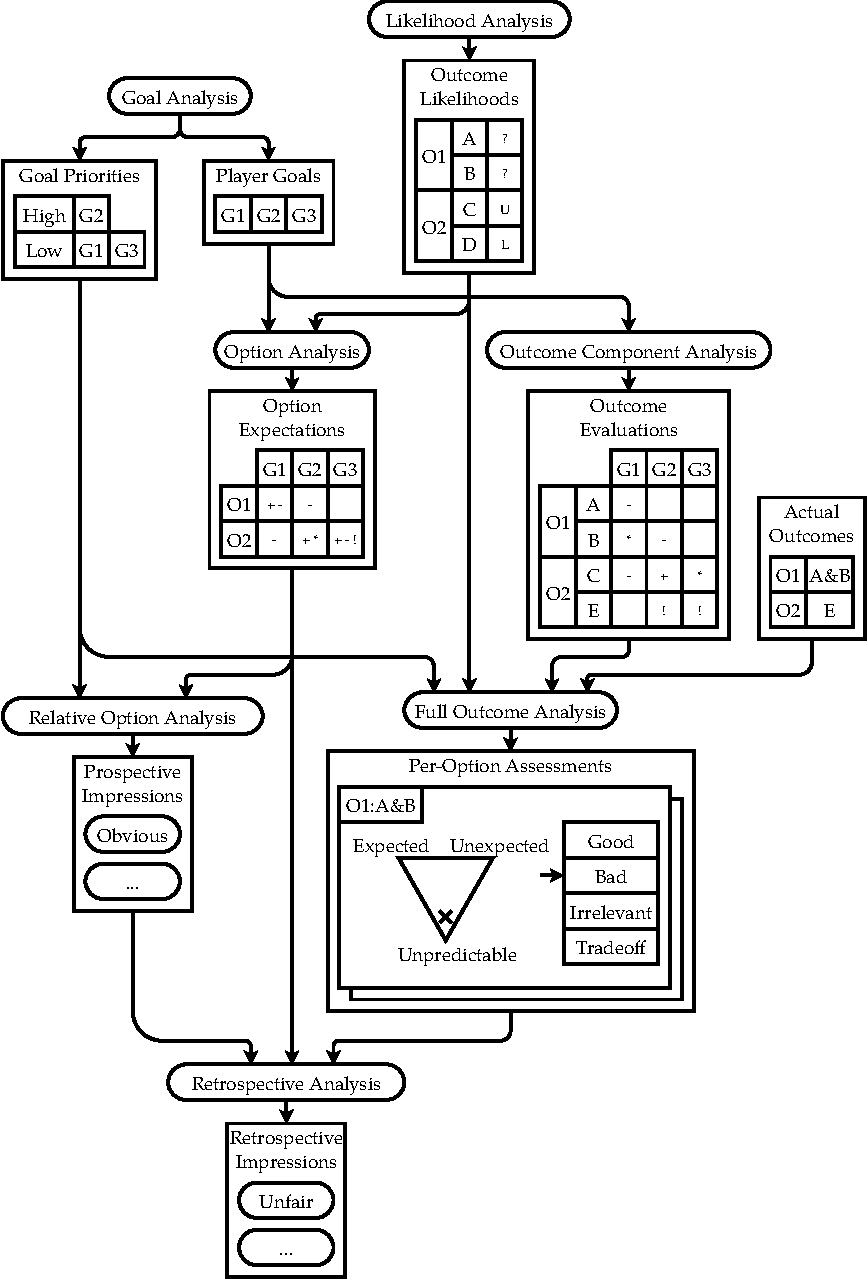
\includegraphics[width=0.45\textwidth]{fig/analysis-method-crop.pdf}
  }
  &
  \vspace{2em}
  \begin{enumerate}\addtolength{\itemsep}{0.5\baselineskip}
    \item Goal Analysis
    \item Likelihood Analysis
    \item Option Analysis
    \item Relative Option Analysis
    \item Outcome Component Analysis
    \item Full Outcome Analysis
    \item Retrospective Analysis
  \end{enumerate}
  \end{tabular}
\end{frame}

\begin{frame}{1. Goal Analysis}
  \begin{itemize}\addtolength{\itemsep}{0.5\baselineskip}
    \item Come up with an estimate of the player's goals. 
    \item Also estimate goal priorities.
    \item Without online player modelling, an authorial estimate of player goals must sufice.
    \item Multiple independent analyses can capture player groups with different modes of engagement.
  \end{itemize}
\end{frame}

\begin{frame}{An Example}
  \centering
  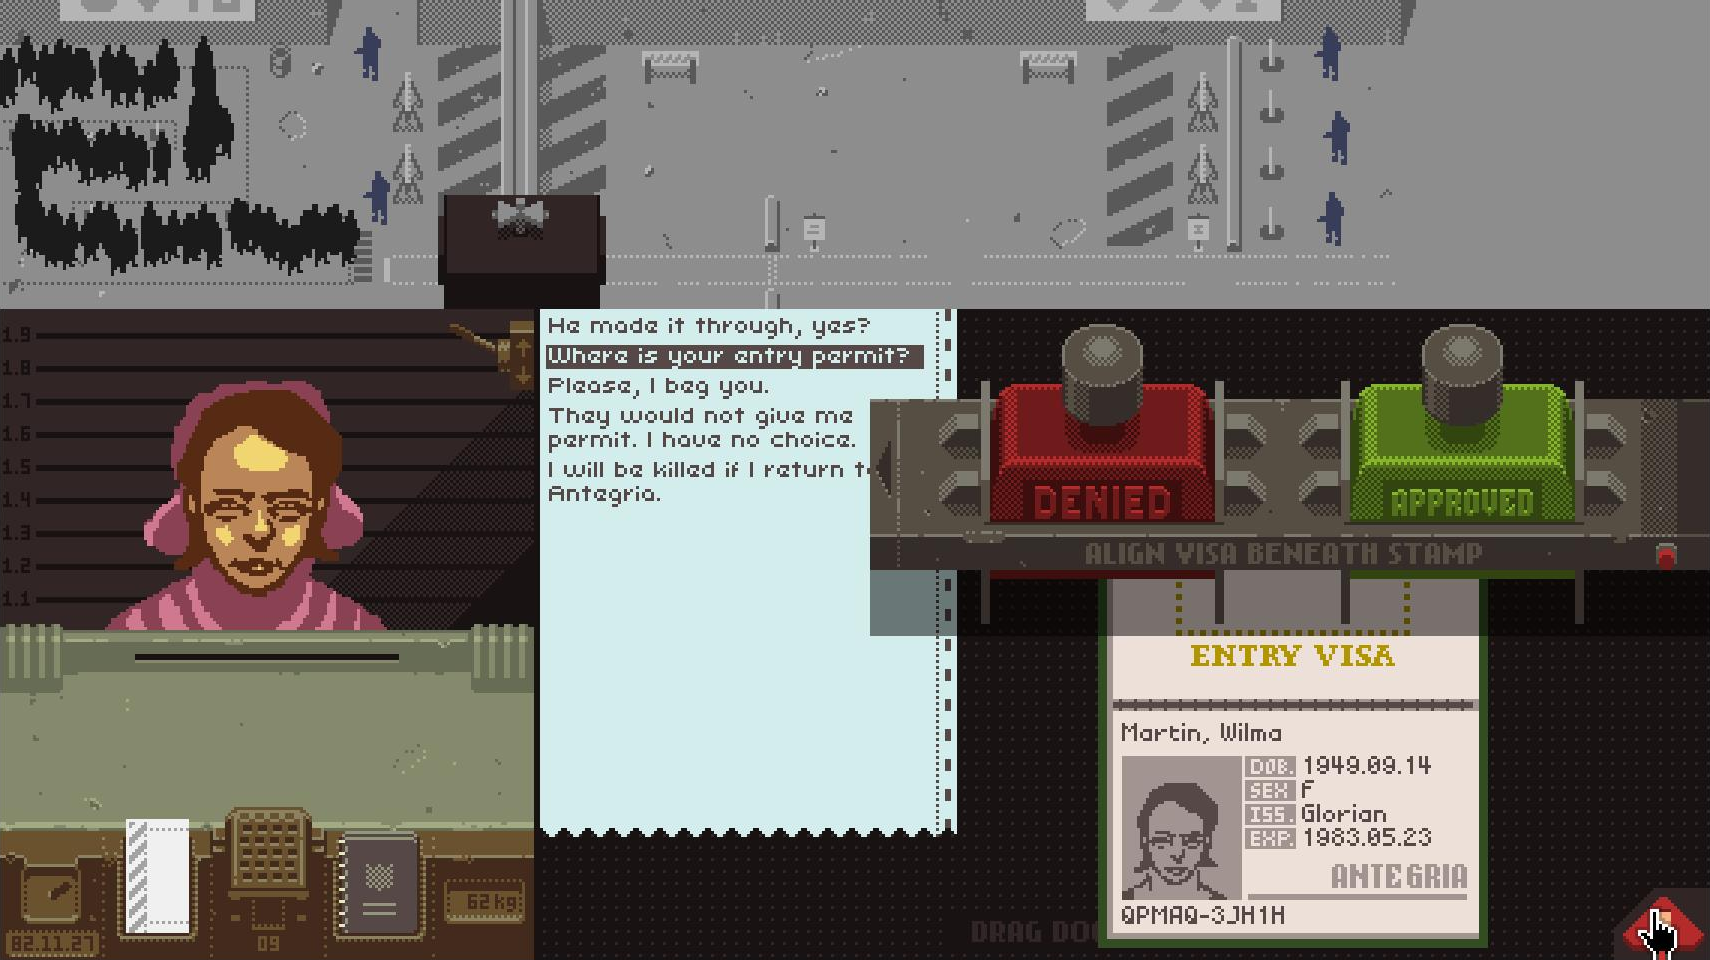
\includegraphics[width=\textwidth]{res/papersplease-large.png} \\
\end{frame}

\begin{frame}{Example: Goal Analysis}
  \centering
  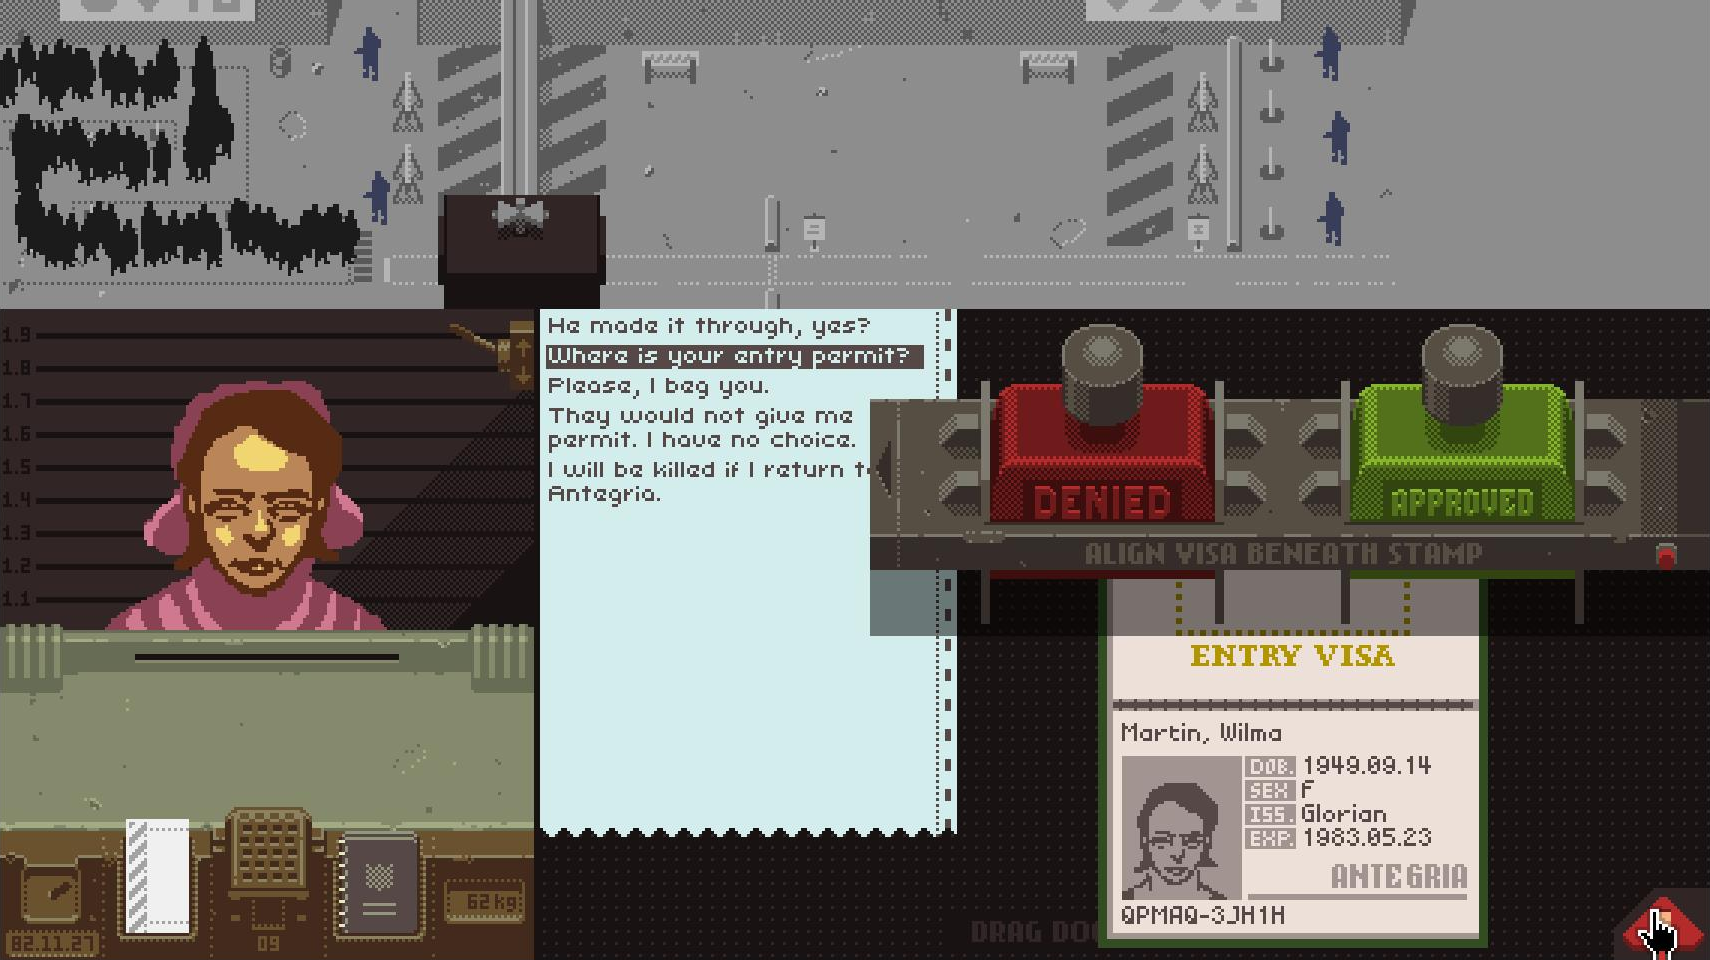
\includegraphics[height=0.3\textheight]{res/papersplease-large.png} \\
  \raggedright
  \begin{itemize}
    \item {[highest] Feed your family.}
    \item {[high] Avoid the penalty for making mistakes.}
    \item {[high] Treat travelers ethically.}
    \item {[medium] Prevent dishonest travelers from gaining entry.}
    \item {[low] Let approved travelers through.}
  \end{itemize}
\end{frame}

\begin{frame}{2. Likelihood Analysis}
  \begin{itemize}\addtolength{\itemsep}{0.5\baselineskip}
    \item Estimate the likelihood of each outcome component of every option.
    \item Only necessary when outcomes are nondeterministic.
    \item Estimate likelihoods \emph{from the player's perspective}.
    \item Again, multiple independent analyses can capture different player perspectives.
  \end{itemize}
\end{frame}

\begin{frame}{Example: Likelihood Analysis}
  \centering
  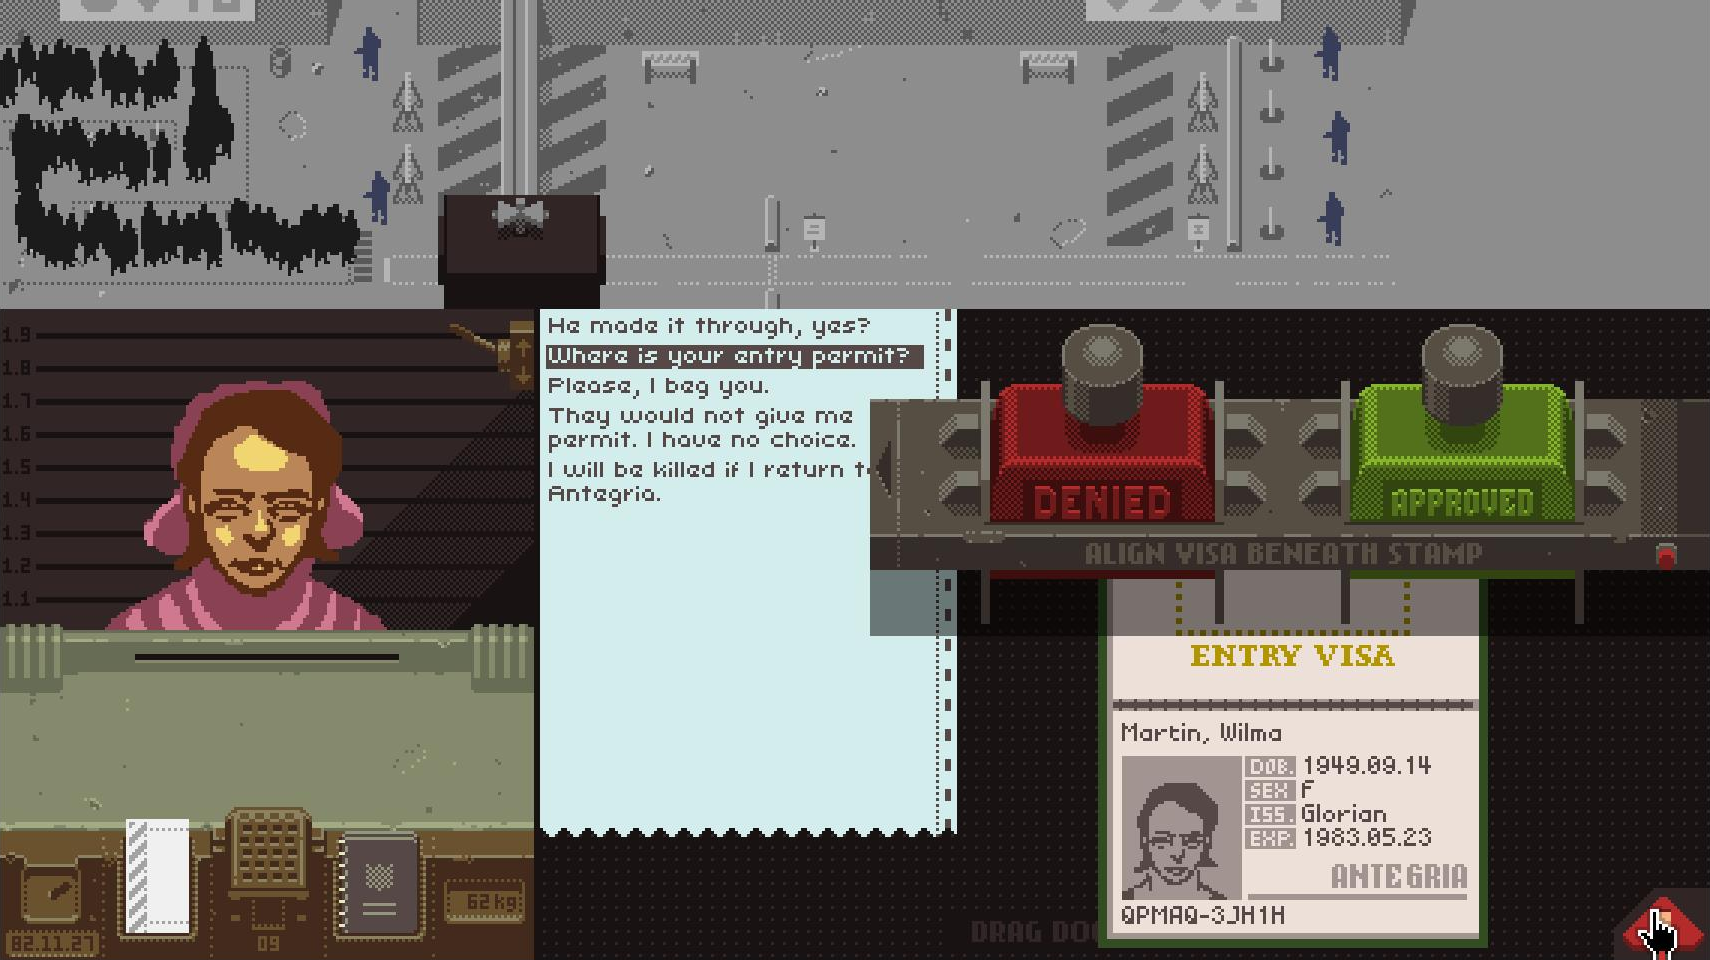
\includegraphics[height=0.3\textheight]{res/papersplease-large.png} \\
  \vspace*{1em}
  \small
  \begin{tabular}{l l}
    \toprule
    \multicolumn{1}{c}{\textbf{Approve}} & \multicolumn{1}{c}{\textbf{Deny}} \\
    \midrule
    {[likely] `Mistake' is discovered.} & [likely] No mistake is possible. \\
    {[unknown] Traveler is saved.} & [unknown] Traveler will be killed. \\
    {[unknown] Crminal gains entry.} & [unknown] Criminal is stymied. \\
    {[unlikely] Earn a credit.} & [likely] Earn a credit. \\
    \bottomrule
  \end{tabular}
\end{frame}

\begin{frame}{3. Option Analysis}
  \begin{itemize}\addtolength{\itemsep}{0.5\baselineskip}
    \item Given outcome likelihoods and player goals, estimate the perceived effect of each option on each goal.
    \item Per option/goal, look for positive or negative effects and whether they're likely or merely possible.
  \end{itemize}
  \vfill
  \centering
  \begin{tabular}{r c c}
    \toprule
           & Possible & Likely \\
    \midrule
    Positive    & \textbf{Enables}  & \textbf{Advances} \\
    Negative & \textbf{Threatens} & \textbf{Hinders} \\
    \bottomrule
  \end{tabular}
  \vfill
  \raggedright
  \begin{itemize}\addtolength{\itemsep}{0.5\baselineskip}
    \item Multiple overlapping assignments are possible (e.g., a choice that \textbf{enables}, \textbf{threatens}, \emph{and} \textbf{hinders} a particular goal).
  \end{itemize}
\end{frame}

\begin{frame}{Example: Option Analysis}
  \centering
  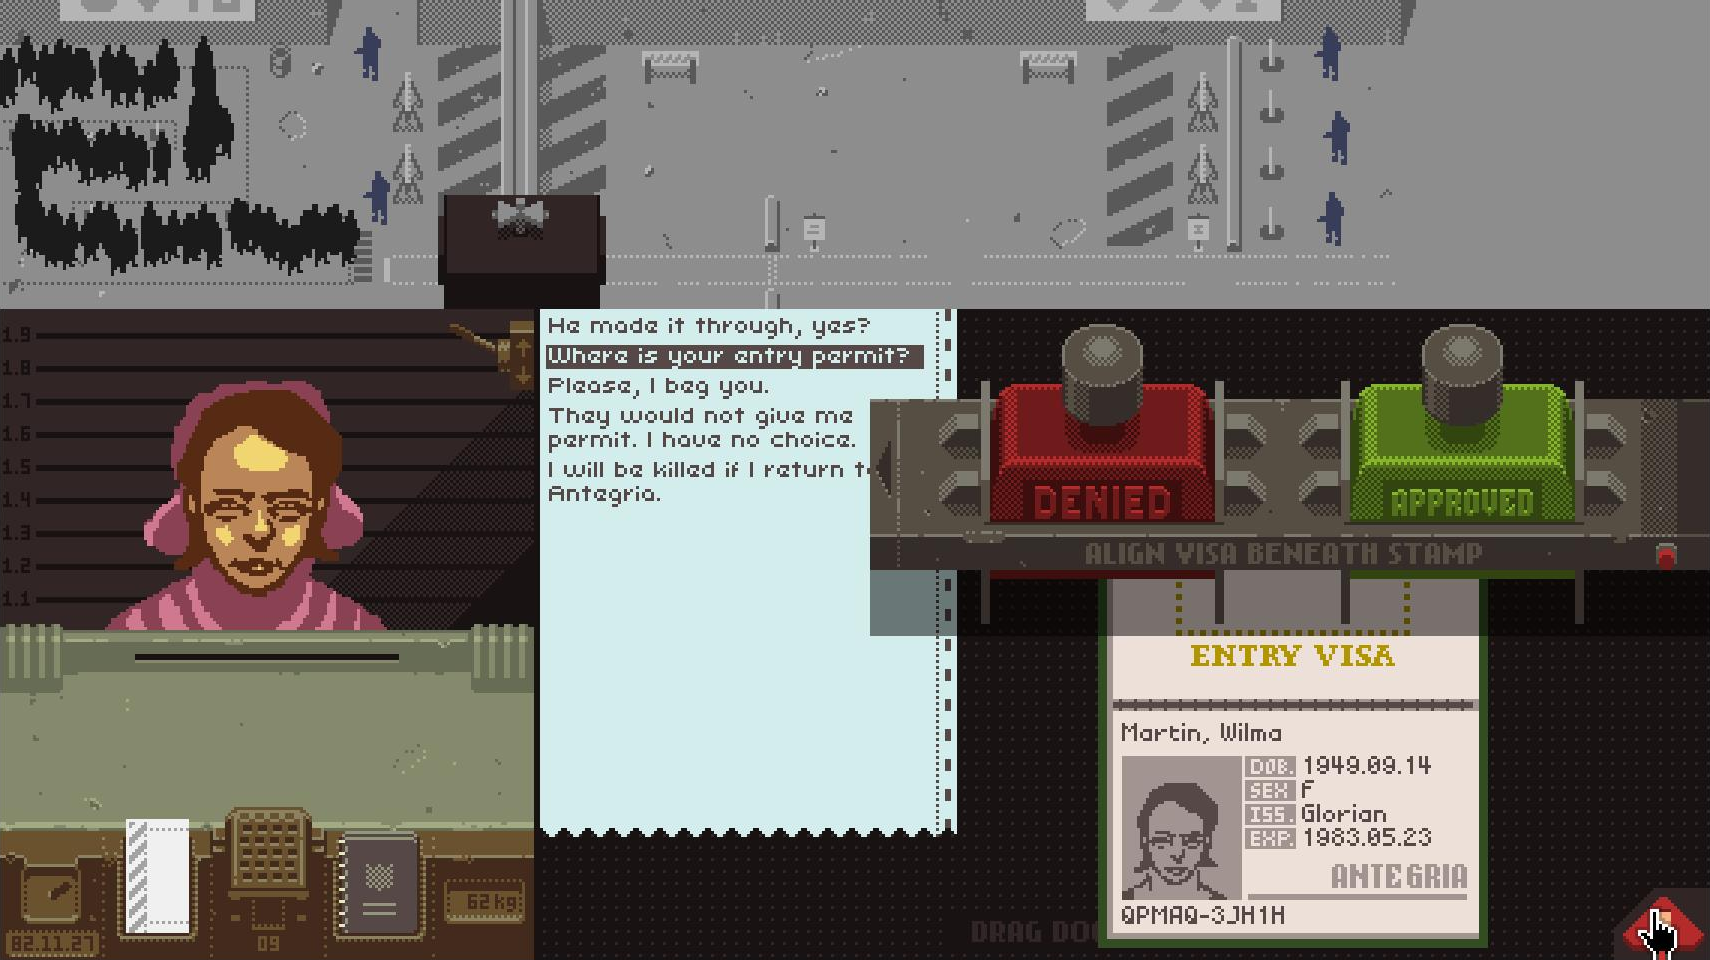
\includegraphics[height=0.3\textheight]{res/papersplease-large.png} \\
  \vspace*{0.2em}
  \footnotesize
  \begin{tabular}{c c c}
    \toprule
    \textbf{Goal} & \textbf{Approve} & \textbf{Deny} \\
    \midrule
    \multirow{3}{*}{<feed your family>} & \textbf{enables} & \textbf{enables} \\
                                        & \textbf{threatens} & \\
                                        & \textbf{hinders} & \textbf{advances} \\
    \midrule

    \multirow{3}{*}{<avoid penalty>} & \textbf{enables} & \textbf{enables} \\
                                     & \textbf{threatens} & \\
                                     & \textbf{hinders} & \textbf{advances} \\
    \midrule

    \multirow{2}{*}{<treat ethically>} & \textbf{enables} & \textbf{enables} \\
                                       & & \textbf{threatens} \\
    \midrule

    <stop cheaters> & \textbf{threatens} & \textbf{enables} \\
    \bottomrule
  \end{tabular}
\end{frame}

\begin{frame}{4. Relative Option Analysis}
  \begin{itemize}\addtolength{\itemsep}{0.5\baselineskip}
    \item Given goal priorities and the results of option analysis, categorize the set of options.
    \item Some structures such as a \textbf{dilemma} or an \textbf{obvious} choice may be immediately recognizeable.
    \item Other structures can be compared to well-understood cases.
  \end{itemize}
\end{frame}

\begin{frame}{4. Relative Option Analysis}
\centering
\renewcommand*{\arraystretch}{1.5}
\footnotesize
\hspace*{-1.5em}
\begin{tabular}{p{4.5em}p{10em}p{18.5em}}
\toprule
\textbf{Label} & \textbf{Description} & \textbf{Criteria} \\
\midrule
\textbf{Dilemma} & A difficult decision between two negative outcomes. & Exactly two options, each of which \textbf{hinders} one of two different high-priority player goals. The priorities of the goals and the severity of the consequences should be balanced and neither option should \textbf{enable} or \textbf{advance} any goals (even low-priority ones). \\
\textbf{Obvious} & A choice that has one option which is clearly better than the rest. & One option that \textbf{advances} a high-priority player goal without \textbf{hindering} any (although it may \textbf{threaten} some), while none of the rest of the options \textbf{enable} any high-priority goals, and each of them \textbf{threatens} some goal. \\
\textbf{Relaxed} & A choice that has no impact on any high-priority goals and where no goals are threatened. & There are no option expectations involving high-priority goals (positive or negative), and there are no \textbf{threatens} expectations (and thus no \textbf{hinders} expectations). \\
\bottomrule
\end{tabular}
\end{frame}

\begin{frame}{4. Relative Option Analysis}
  \vfill
  \begin{itemize}\addtolength{\itemsep}{0.5\baselineskip}
    \item Only \emph{expected} outcomes are considered, not \emph{actual} outcomes.
    \item Resulting \textbf{prospective impressions} estimate players' perceptions of a choice before making a decision
    \item Some effects such as elevated tension via a series of difficult choices depend mainly on \textbf{prospective impressisons}.
  \end{itemize}
  \vfill
  \centering
  \scriptsize (My first experiment tested the \textbf{relaxed}, \textbf{obvious}, and \textbf{dilemma} impressions.)
\end{frame}

\begin{frame}{Example: Relative Option Analysis}
  \centering
  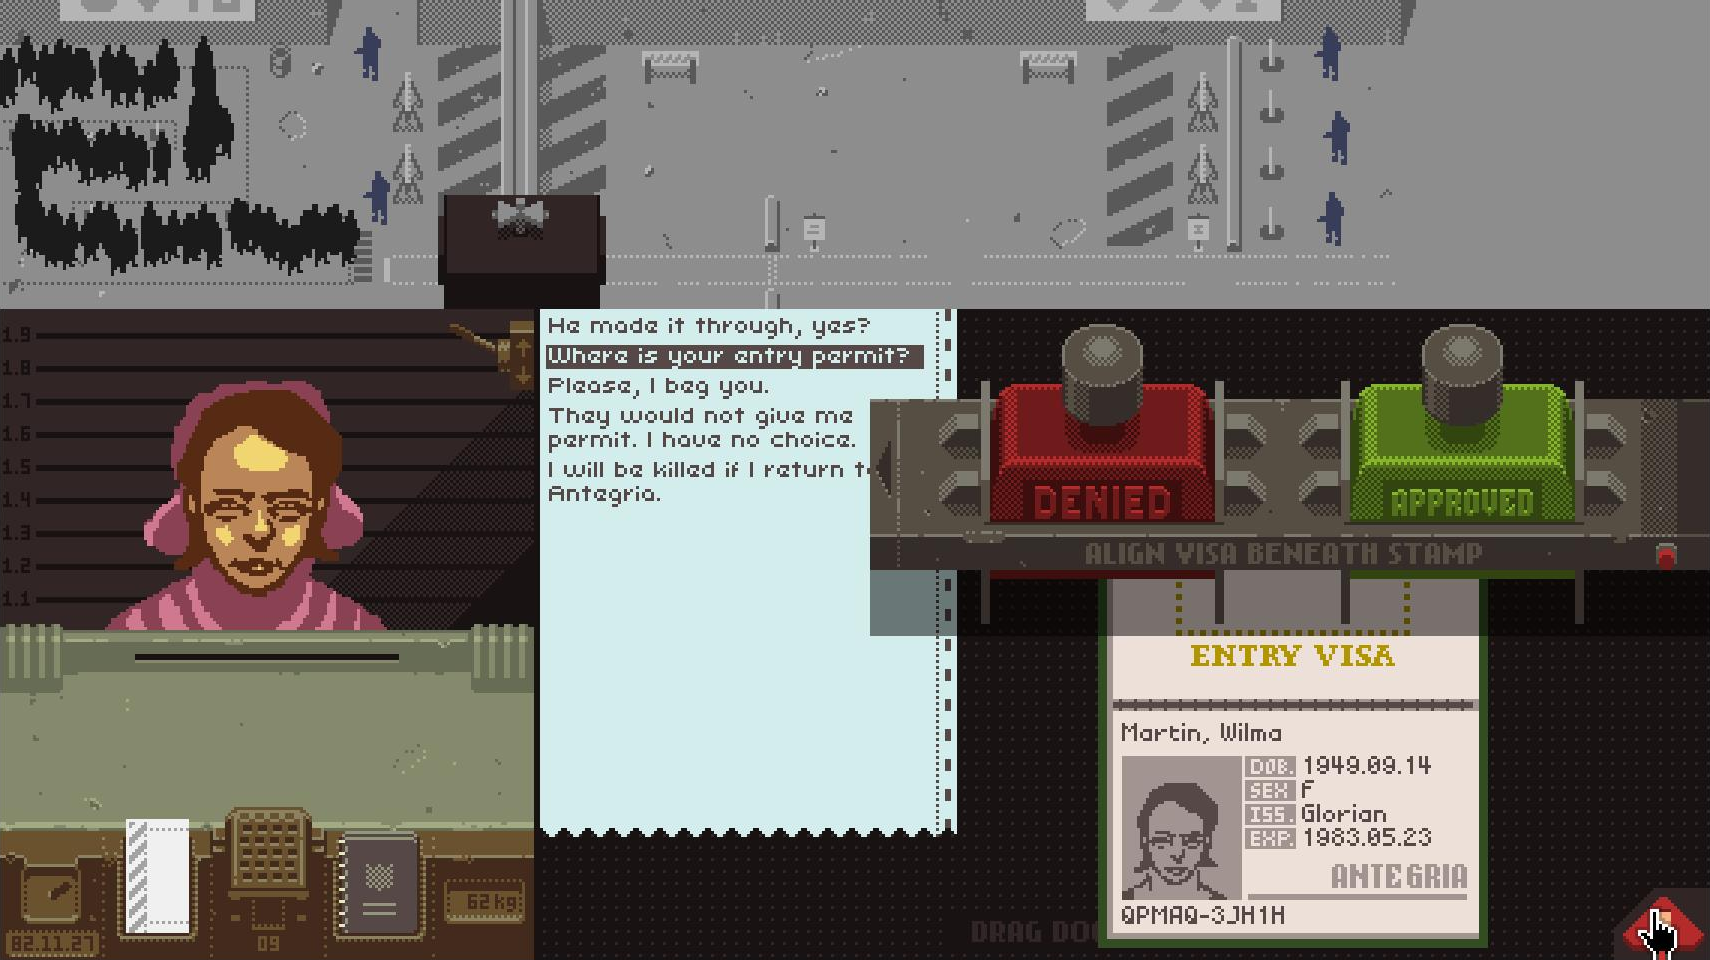
\includegraphics[height=0.3\textheight]{res/papersplease-large.png} \\
  \vspace*{0.2em}
  \footnotesize
  \begin{tabular}{c c c}
    \toprule
    \textbf{Goal} & \textbf{Approve} & \textbf{Deny} \\
    \midrule
    \multirow{3}{*}{<feed your family>} & \textbf{enables} & \textbf{enables} \\
                                        & \textbf{threatens} & \\
                                        & \textbf{hinders} & \textbf{advances} \\
    \midrule

    \multirow{3}{*}{<avoid penalty>} & \textbf{enables} & \textbf{enables} \\
                                     & \textbf{threatens} & \\
                                     & \textbf{hinders} & \textbf{advances} \\
    \midrule

    \multirow{2}{*}{<treat ethically>} & \textbf{enables} & \textbf{enables} \\
                                       & & \textbf{threatens} \\
    \midrule

    <stop cheaters> & \textbf{threatens} & \textbf{enables} \\
    \bottomrule
  \end{tabular}
\end{frame}

\begin{frame}{Example: Relative Option Analysis}
  \centering
  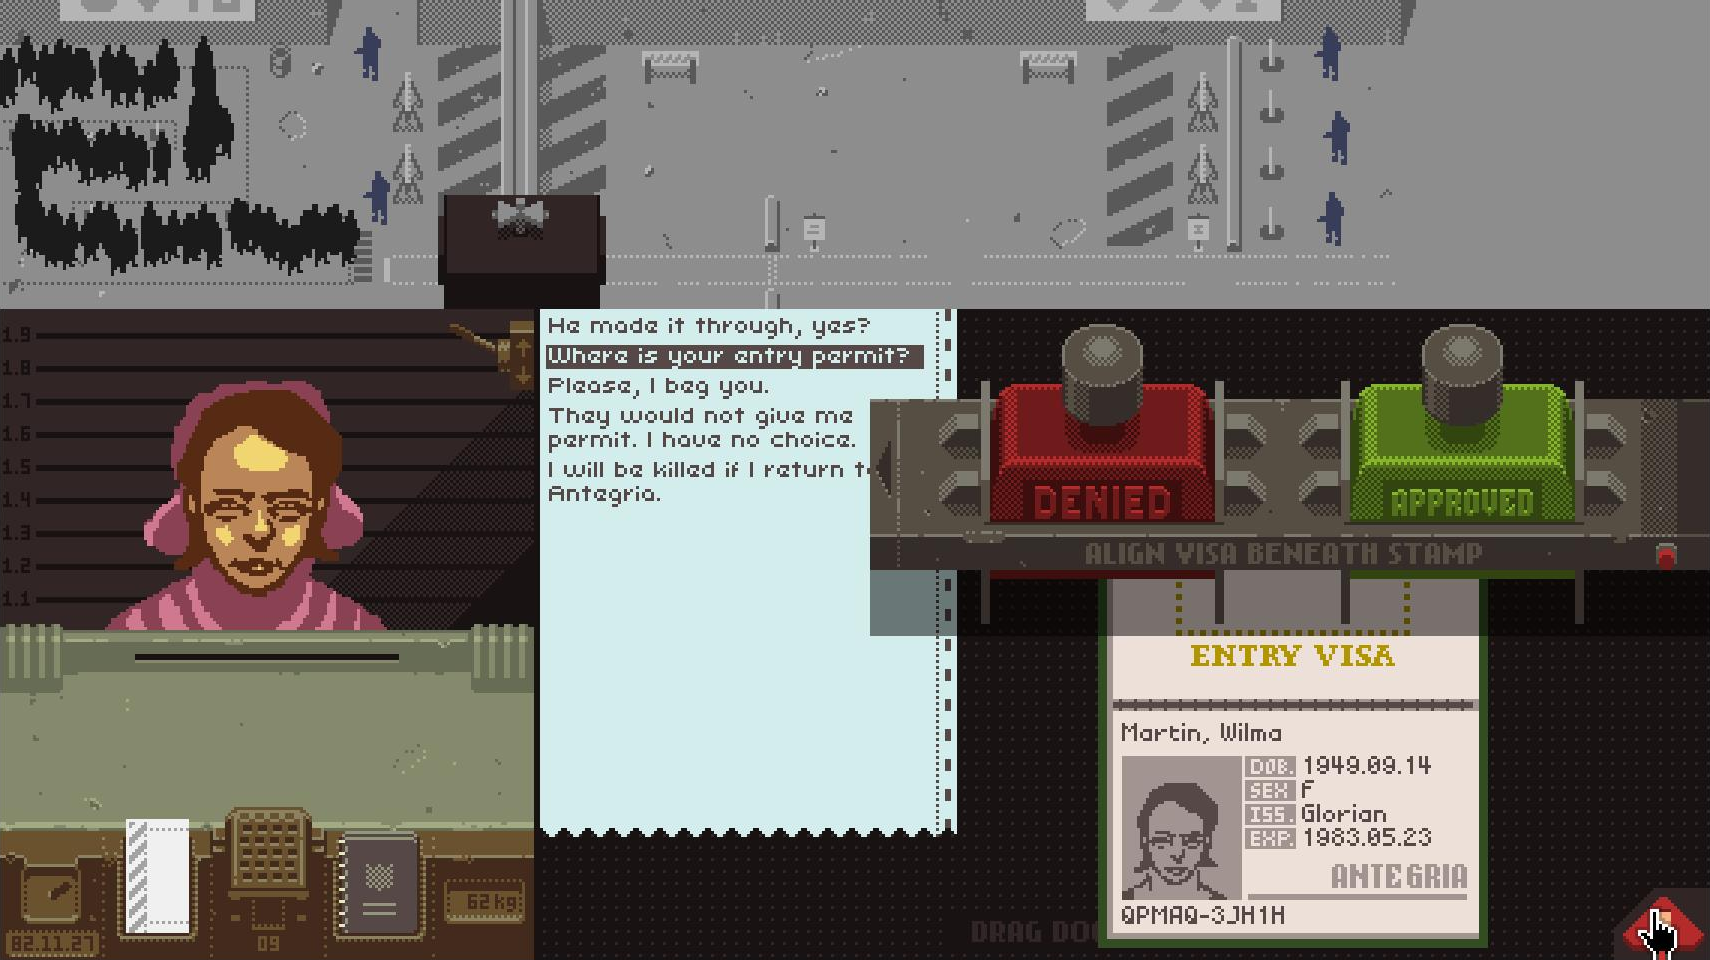
\includegraphics[height=0.3\textheight]{res/papersplease-large.png} \\
  \vspace*{1em}
  \footnotesize
  \begin{tabular}{c c c c c}
    \toprule
    &  \multicolumn{2}{c}{\textit{Doubtful}} & \multicolumn{2}{c}{\textit{Trusting}} \\
    \midrule
    \textbf{Goal} & \textbf{Approve} & \textbf{Deny} & \textbf{Approve} & \textbf{Deny} \\
    \midrule
    \multirow{2}{*}{<treat ethically>} & \textbf{enables}  & \textbf{enables}   & \textbf{enables}  & \textbf{threatens} \\
                                       &                   & \textbf{threatens} & \textbf{advances} & \textbf{hinders}   \\
    \midrule

    <stop cheaters> & \textbf{threatens} & \textbf{enables} & \emph{none} & \emph{none} \\
    \bottomrule
  \end{tabular}
\end{frame}

\begin{frame}{Example: Relative Option Analysis}
  \centering
  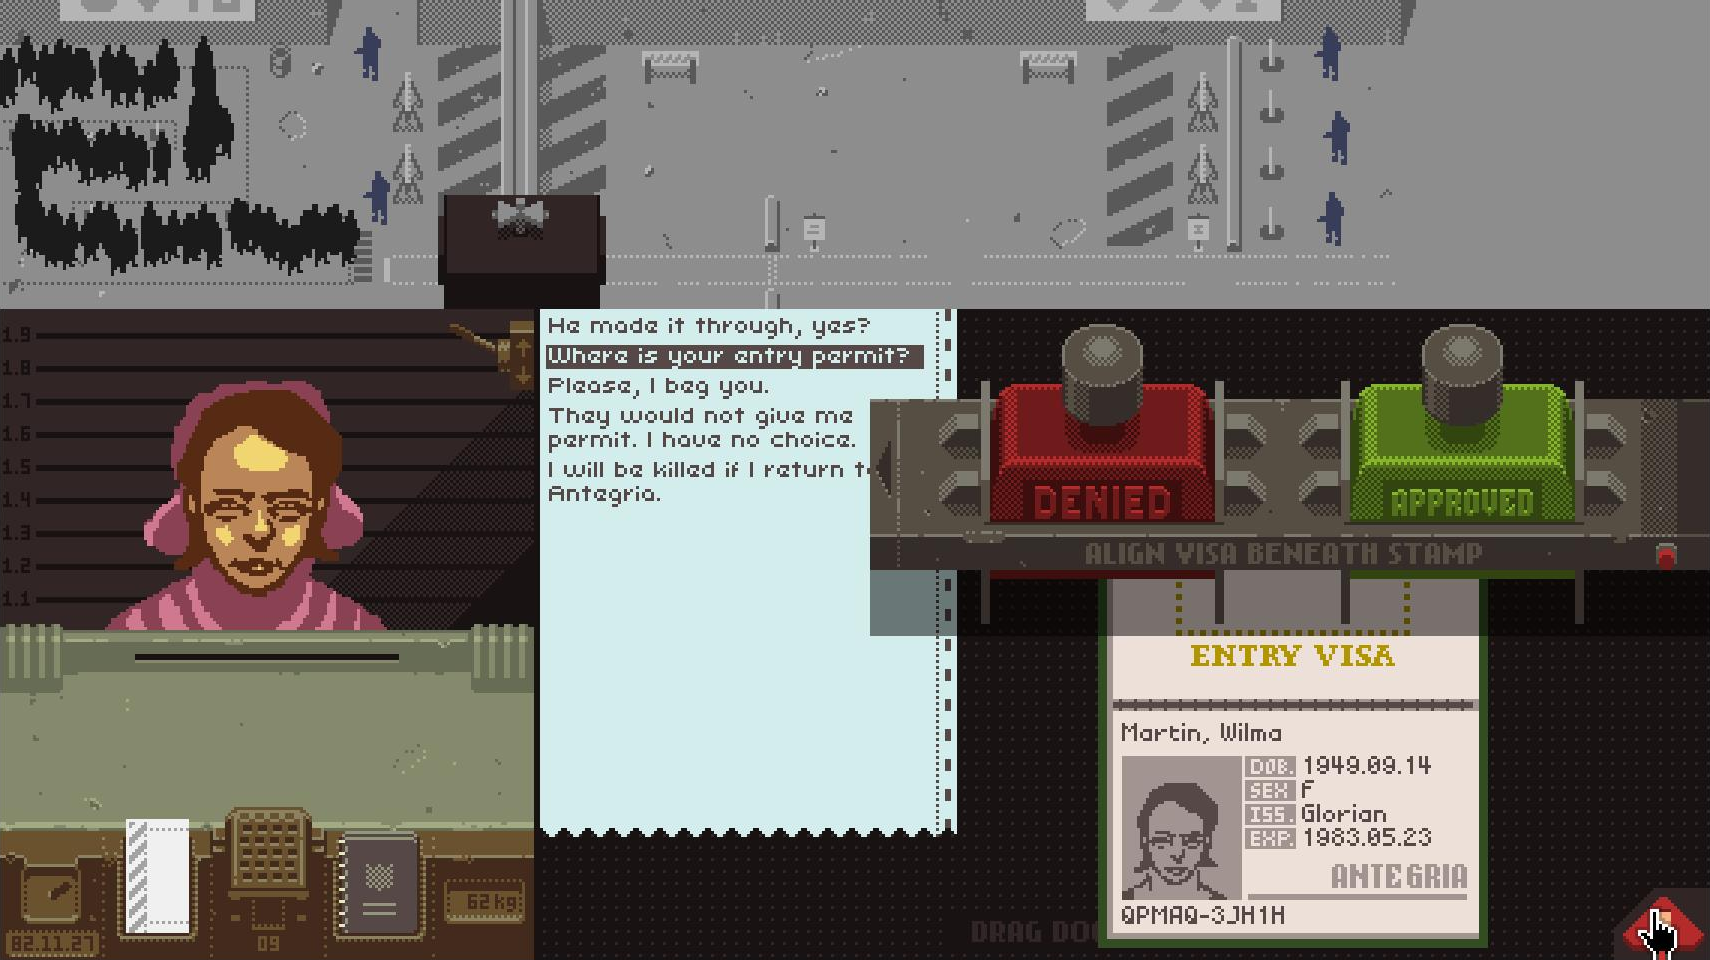
\includegraphics[height=0.3\textheight]{res/papersplease-large.png} \\
  \vspace*{0.5em}
  \footnotesize
  \begin{tabular}{c c c}
    \toprule
    \textbf{Goal} & \textbf{Approve} & \textbf{Deny} \\
    \midrule
    \multirow{3}{*}{<feed your family>} & \textbf{enables} & \textbf{enables} \\
                                        & \textbf{threatens} & \\
                                        & \textbf{hinders} & \textbf{advances} \\
    \midrule

    \multirow{3}{*}{<avoid penalty>} & \textbf{enables} & \textbf{enables} \\
                                     & \textbf{threatens} & \\
                                     & \textbf{hinders} & \textbf{advances} \\
    \midrule

    \multirow{2}{*}{<treat ethically>} & \textbf{enables} & \textbf{threatens} \\
                                       & \textbf{advances} & \textbf{hinders} \\
    \bottomrule
  \end{tabular}
\end{frame}

\begin{frame}{Example: Relative Option Analysis}
  \centering
  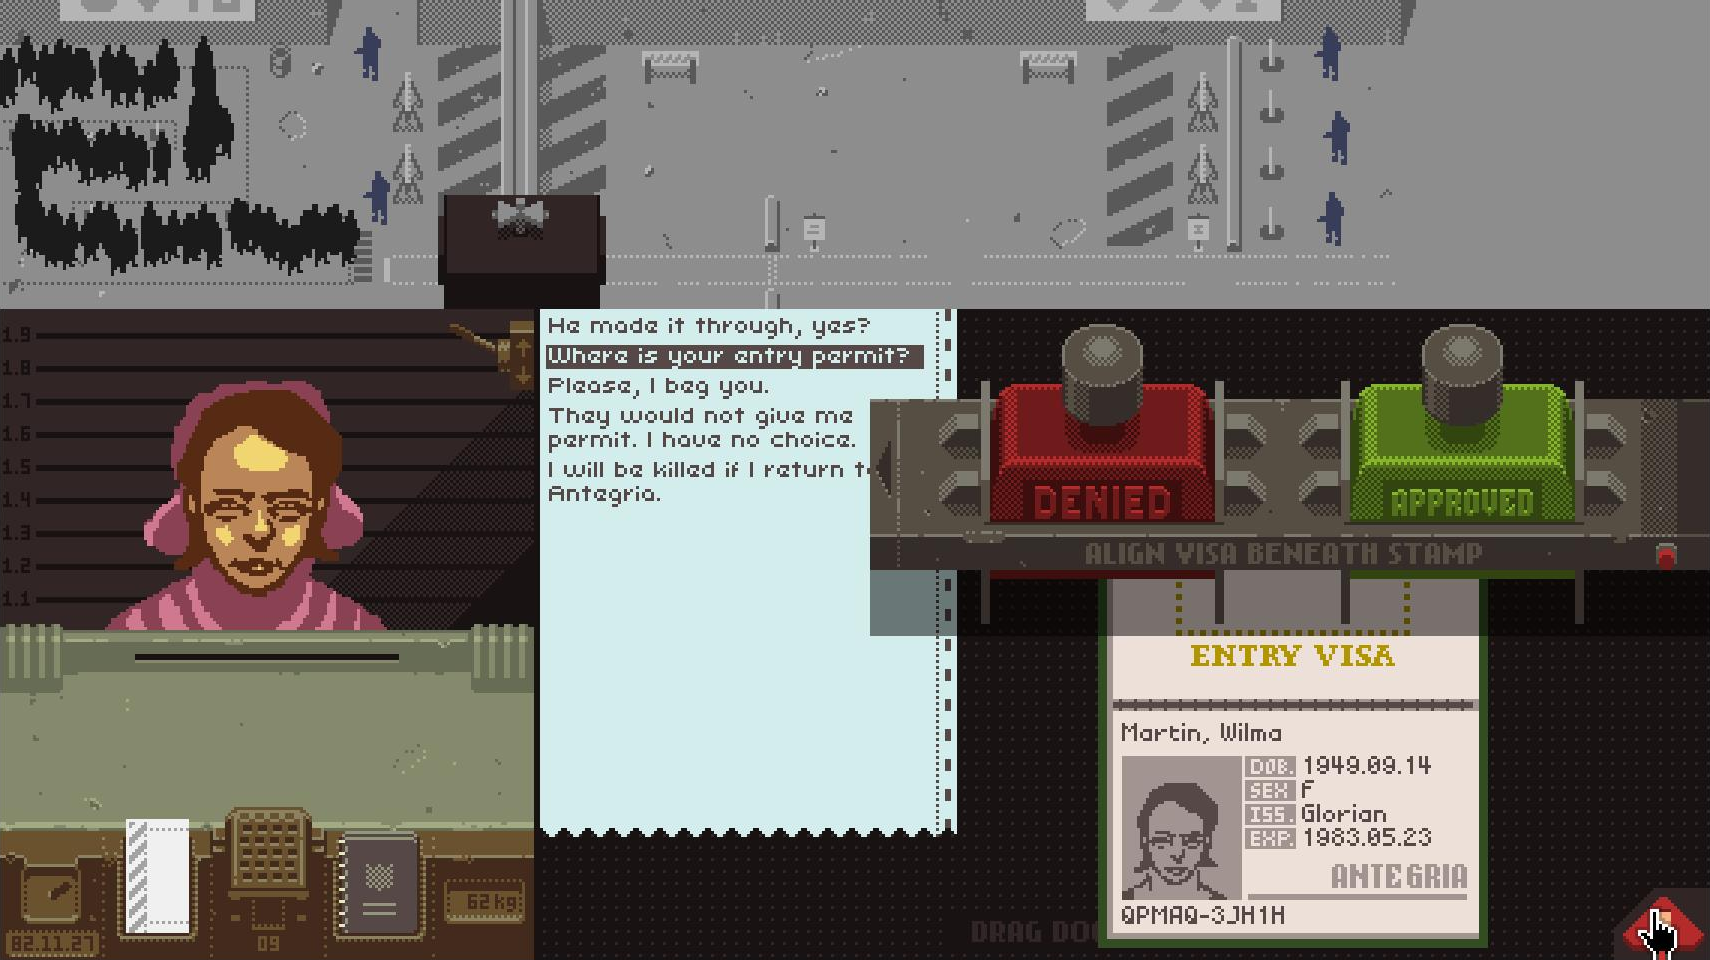
\includegraphics[height=0.3\textheight]{res/papersplease-large.png} \\
  \vspace*{0.5em}
  \footnotesize
  \begin{tabular}{c c c}
    \toprule
    \textbf{Goal} & \textbf{Approve} & \textbf{Deny} \\
    \midrule
    \multirow{3}{*}{<feed your family>} & \textbf{enables} & \textbf{enables} \\
                                        & \textbf{threatens} & \\
                                        & \underline{\textbf{hinders}} & \textbf{advances} \\
    \midrule

    \multirow{3}{*}{<avoid penalty>} & \textbf{enables} & \textbf{enables} \\
                                     & \textbf{threatens} & \\
                                     & \underline{\textbf{hinders}} & \textbf{advances} \\
    \midrule

    \multirow{2}{*}{<treat ethically>} & \textbf{enables} & \textbf{threatens} \\
                                       & \textbf{advances} & \underline{\textbf{hinders}} \\
    \bottomrule
  \end{tabular}
\end{frame}

\begin{frame}{Example: Relative Option Analysis}
  \centering
  \textbf{Dilemma} \\
  \vspace{0.5\baselineskip}
  \raggedright
Exactly two options, each of which \textbf{hinders} one of two different high-priority player goals.
%
The priorities of the goals and the severity of the consequences should be balanced and neither option should \textbf{enable} or \textbf{advance} any goals (even low-priority ones).
\end{frame}

\begin{frame}{Example: Prospective Impression}
  \centering
  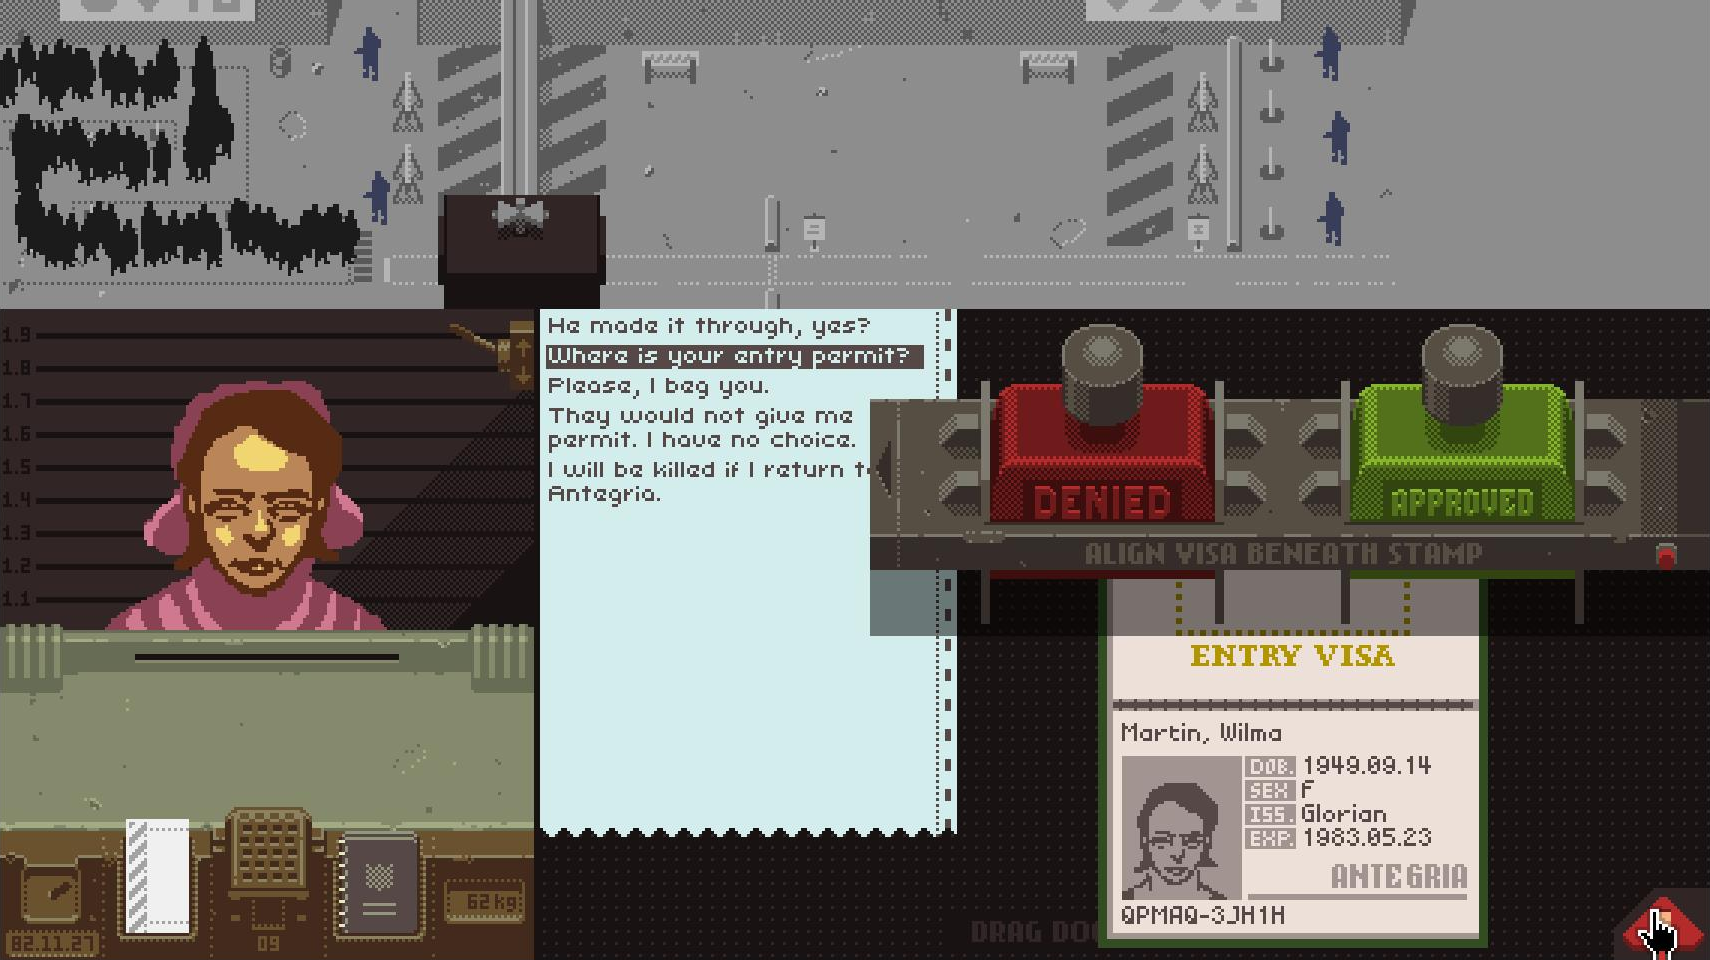
\includegraphics[width=0.9\textwidth]{res/papersplease-large.png} \\
  \vspace{1em}
  \pause
  \textbf{dilemma + doubt = complicity}
\end{frame}

\begin{frame}{5. Outcome Component Analysis}
  \begin{itemize}\addtolength{\itemsep}{0.5\baselineskip}
    \item The impact of each actual outcome component on each player goal is considered.
    \item Major/minor positive/negative labels may be used, or some finer scale of good/bad impacts.
    \item The \emph{suggested} outcome components from the likelihood analysis step may not be \emph{actual}.
    \item There may also be \emph{non-suggested} \emph{actual} outcome components.
    \item In some cases, probability can be folded into severity.
  \end{itemize}
\end{frame}

\begin{frame}{6. Full Outcome Analysis}
  \begin{itemize}\addtolength{\itemsep}{0.5\baselineskip}
    \item Information from goal analysis, likelihood analysis, and outcome component analysis is combined.
    \item Entire outcomes are categorized as \textbf{good}, \textbf{bad}, \textbf{irrelevant} or \textbf{tradeoffs} according to the effects their components have on various goals.
    \item Outcomes are also categorized as \textbf{expected}, \textbf{unexpected}, or \textbf{unpredictable} based on comparing the results of likelihood analysis with the results of outcome component analysis.
    \item These \emph{valence} and \emph{expectedness} values give a wholistic view of the outcome of each option.
  \end{itemize}
\end{frame}

\begin{frame}{7. Retrospective Analysis}
  \begin{itemize}\addtolength{\itemsep}{0.5\baselineskip}
    \item Estimates \textbf{retrospective impressions} using information from relative option analysis and full outcome analysis.
    \item Different options usually have different \textbf{retrospective impressions}.
    \item As with the \textbf{prospective impression} of an entire choice, exemplars such as \textbf{miracle} or \textbf{unfair} anchor the analysis.
  \end{itemize}
  \vfill
  \centering
  \scriptsize (My second experiment tested the \textbf{expected success}, \textbf{expected failure}, \textbf{unfair}, and \textbf{miracle} impressions.)
\end{frame}

\begin{frame}{7. Retrospective Analysis}
\centering
\renewcommand*{\arraystretch}{1.5}
\footnotesize
\hspace*{-1.5em}
\begin{tabular}{p{4.5em}p{12em}p{16.5em}}
\toprule
\textbf{Label} & \textbf{Description} & \textbf{Criteria} \\
\midrule
\textbf{Expected Success} & A predictable outcome that advances player goals. & The option selected \textbf{advances} a player goal without \textbf{hindering} any, and its outcome is both \textbf{predictable} and \textbf{good}. \\
\textbf{Unfair} & An option that seemed good but had unexpected negative consequences. & The selected option must be expected to \textbf{advance} at least one high-priority player goal, while not \textbf{hindering} any. It must also have an \textbf{unexpected} and \textbf{bad} outcome. \\
\textbf{Miracle} & An option that seemed like a lost cause but that unexpectedly turned out well. & The selected option must be expected to \textbf{fail} at least one high-priority goal, while not \textbf{advancing} any. It must have an \textbf{unexpected} and \textbf{good} outcome. \\
\bottomrule
\end{tabular}
\end{frame}

\begin{frame}{Outline}
  \begin{itemize}
    \item Motivation
    \item Inspiration: \skald/ and \problemplanets/
    \item Methodology
    \item Related Work
    \item Theory: Choice Poetics
    \item \textbf{Application: \dunyazad/}
    \item \textbf{Results: Options}
    \item \textbf{Results: Outcomes}
    \item \textbf{Conclusions}
  \end{itemize}
\end{frame}

\begin{frame}{\dunyazad/}
  \begin{itemize}\addtolength{\itemsep}{0.5\baselineskip}
    \item \dunyazad/ is an operationalization of goal-based choice analysis.
    \item Using answer set programming, it solves for choice structures with specified prospective and retrospective impressions.
    \item Imperative code can chain these choices together into an interactive story.
    \item Choice structures are converted into English text and code (HTML or similar).
  \end{itemize}
\end{frame}

\begin{frame}{Constraints}
  \begin{itemize}\addtolength{\itemsep}{0.5\baselineskip}
    \item \textbf{Representational constraints} define the basic elements of choices.
    \item \textbf{Constitutent constraints} define how those elements come together to form choices.
    \item \textbf{Aesthetic constraints} limit the kinds of configurations allowed to those that make sense.
    \item \textbf{Poetic constraints} distinguish between allowed configurations and permit users to request specific impressions.
  \end{itemize}
\end{frame}

\begin{frame}{State Representation}
  \centering
  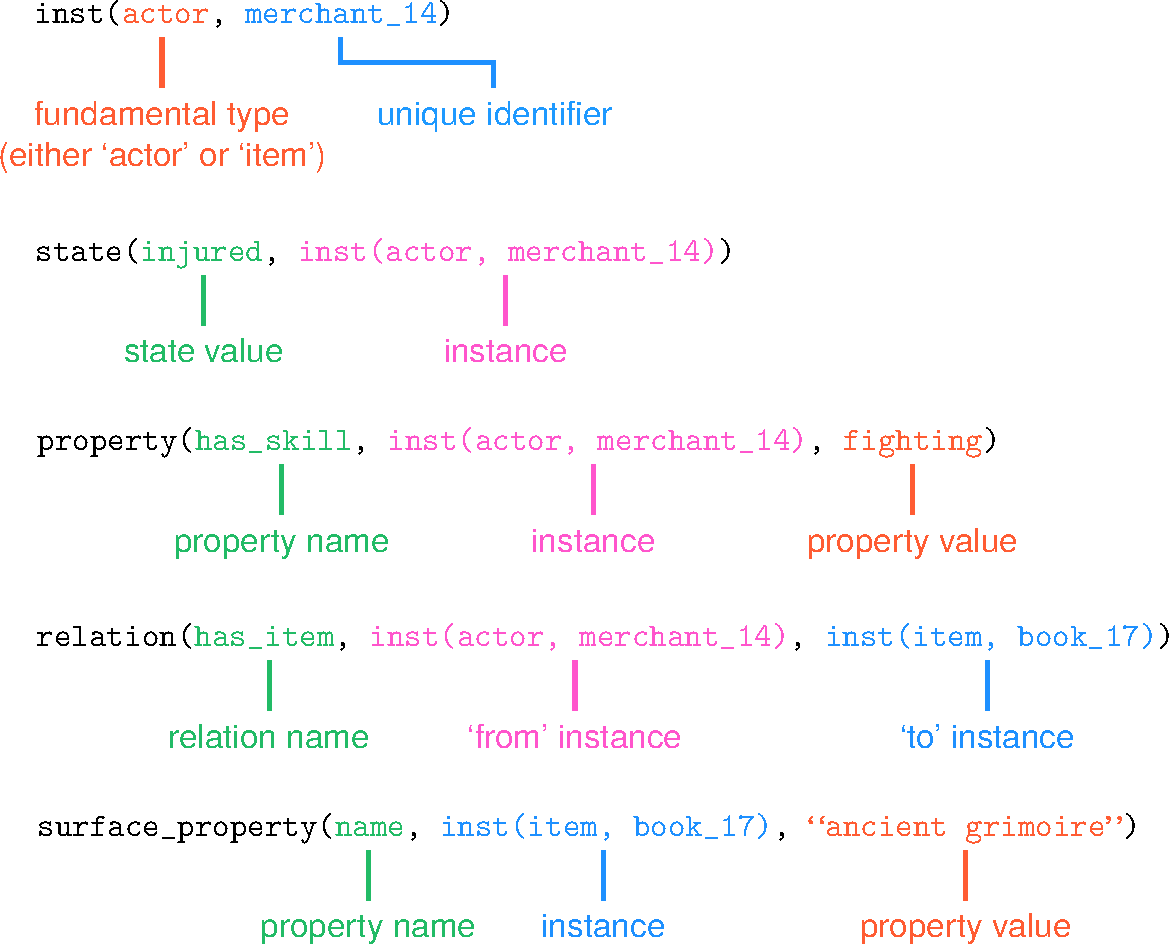
\includegraphics[height=0.8\textheight]{fig/cropped-dunyazad-states.pdf}
\end{frame}

\begin{frame}{State Representation}
  \centering
\fbox{%
\parbox{\textwidth}{
  \small
Scene:\svind\\
\ind ``A merchant carrying some perfume is being threatened by bandits.''\vind\\
Representation:\svind \\
\ind \parbox{0.9\textwidth}{ \tt
\scriptsize
inst(actor,businessperson\_4). \\
inst(actor,tough\_3). \\
inst(item,treasure\_5). \\
property(type,inst(actor,businessperson\_4),merchant). \\
property(type,inst(actor,tough\_3),bandits). \\
property(type,inst(item,treasure\_5),perfume). \\
relation( \\
\ind has\_item, \\
\ind inst(actor,businessperson\_4), \\
\ind inst(item,treasure\_5) \\
). \\
relation( \\
\ind threatening, \\
\ind inst(actor,tough\_3), \\
\ind inst(actor,businessperson\_4) \\
). \\
surface\_property(name,inst(item,treasure\_5),"perfume").
}
}
}
\end{frame}

\begin{frame}{Action Representation}
  \begin{itemize}\addtolength{\itemsep}{0.5\baselineskip}
    \item Each state has one or more options, which lead to other states.
    \item Each option corresponds to an action, with variable pre- and post-conditions.
    \item Effects of an action are split across outcome components, for example \prq{victory}{,} \prq{defeat}{,} and \prq{draw}{} for the \prq{attack}{} action.
    \item Outcome components may be exclusive, and each may have its own preconditions.
    \item At each option, the active outcome components are fixed, and the corresponding state changes are recorded as consequences.
  \end{itemize}
\end{frame}

\begin{frame}{Action Inventory}
\vfill
\centering
\renewcommand*{\arraystretch}{1.5}
\footnotesize
\hspace*{-1.5em}
\begin{tabular}{c c c c}
  \pr{accuse}       & \pr{explain\_innocence} & \pr{play\_song}         & \pr{talk\_down} \\
  \cg{\pr{arrive}*}       & \pr{flee}               & \pr{polymorph}          & \pr{tell\_story} \\
  \pr{attack}       & \pr{gossip}             & \cg{\pr{pursue}*}             & \pr{trade} \\
  \pr{buy\_healing} & \pr{leave}              & \pr{reach\_destination} & \pr{travel\_onwards} \\
  \pr{deny\_blame}  & \pr{pacify}             & \pr{shift\_blame}       & \pr{treat\_injury} \\
  \pr{dispel}       & \pr{pay\_off}           & \pr{steal}
\end{tabular}
\vfill
\normalsize
\dunyazad/'s 23 current actions.
\end{frame}

\begin{frame}{Setups}
  \begin{itemize}\addtolength{\itemsep}{0.5\baselineskip}
    \item \dunyazad/ uses \textbf{setups} to create interesting situations.
    \item Each \textbf{setup} includes some variable parts.
    \item Once \textbf{potentials} are resolved, the characters ``travel onwards'' and a new setup is invoked.
    \item Combined with rules for character motivation, \textbf{potentials} drive the action forward.
  \end{itemize}
\end{frame}

\begin{frame}{Constituent Constraints}
  \begin{itemize}\addtolength{\itemsep}{0.5\baselineskip}
    \item Motivation, relevance, repetition, etc.
    \item Likely outcomes based on character skills and tools.
    \item Common-sense rules (e.g., being incapacitated).
  \end{itemize}
\end{frame}

\begin{frame}{Aesthetic Constraints}
  \begin{itemize}\addtolength{\itemsep}{0.5\baselineskip}
    \item Enforce narrative perspective (second person).
    \item Mandate variety and track boredom.
    \item Exclude undesirable configurations (e.g., trick options).
  \end{itemize}
\end{frame}

\begin{frame}{Poetic Constraints}
  \begin{itemize}\addtolength{\itemsep}{0.5\baselineskip}
    \item Each step of goal-based choice analysis is represented.
    \item Goal analysis consists of hand-specified player goals:
    \begin{itemize}\addtolength{\itemsep}{0.5\baselineskip}
      \vspace{0.5\baselineskip}
      \item {[high]}\prq{preserve\_health}{}
      \item {[high]}\prq{avoid\_threats\_to}{}
      \item {[high]}\prq{avoid\_accusations}{}
      \item {[high]}\prq{preserve\_original\_form}{}
      \item {[high]}\prq{reclaim\_property}{}
      \item {[low]}\prq{as\_intended}{}
      \item {[low]}\prq{have\_tool\_for}{}
    \end{itemize}
    \item Skill links are used to determine likelihoods.
  \end{itemize}
\end{frame}

\begin{frame}{Output Example}
  \itshape
You come to a tavern and decide to rest for a while.
%
A merchant is bored and a noble is bored and an innkeeper seems knowledgeable.
%
What do you do?
\begin{enumerate}
\item You play a song for the noble \\
  (You have skill: musician. You have no tool for music).
\item You gossip with the innkeeper \\
  (You are missing skill: negotiation).
\item You play a song for the merchant \\
  (You have skill: musician. You have no tool for music).
\end{enumerate}
\end{frame}

\begin{frame}{Outline}
  \begin{itemize}
    \item Motivation
    \item Inspiration: \skald/ and \problemplanets/
    \item Methodology
    \item Related Work
    \item Theory: Choice Poetics
    \item Application: \dunyazad/
    \item \textbf{Results: Options}
    \item \textbf{Results: Outcomes}
    \item \textbf{Conclusions}
  \end{itemize}
\end{frame}

\begin{frame}{Option Experiment}
  \begin{itemize}\addtolength{\itemsep}{0.5\baselineskip}
    \item An online experiment using choices created by \dunyazad/.
    \item Participants read a choice and then answered questions.
    \begin{itemize}\addtolength{\itemsep}{0.5\baselineskip}
      \vspace{0.5\baselineskip}
      \item 90 Amazon Mechanical Turk workers (+6 rejected).
      \item \$0.50 per task (one per worker).
      \item Median response time was 4:40.
      \item Two questions were used to filter responses and incompletes were removed, leaving 79 valid responses.
      \item The rest of the survey consisted of seven 5-point Likert items.
    \end{itemize}
  \end{itemize}
\end{frame}

\begin{frame}{Experiment Design}
  \begin{itemize}\addtolength{\itemsep}{0.5\baselineskip}
    \item The question: \emph{``Is \dunyazad/ successfully creating the desired prospective impressions?''}
    \pause
    \item $\rightarrow$ \emph{``Are \dunyazad/'s constraints sufficient conditions for the associated poetic effects?''}
    \pause
    \item The \textbf{relaxed}, \textbf{obvious}, and \textbf{dilemma} impressions were used because they cover positive/negative, balanced/imbalanced, and high-/low-stakes options.
    \item \dunyazad/ generated three choices per condition and ten participants saw each choice ($3 \times 3 \times 10 = 90$).
  \end{itemize}
\end{frame}

\begin{frame}{Survey Questions}
  \itshape
  \begin{enumerate}\addtolength{\itemsep}{0.5\baselineskip}
    \item ``There are no bad options at this choice.''
    \item ``There is a clear best option at this choice.''
    \item ``The stakes for this choice are low.''
    \item ``There are no good options at this choice.''
    \item ``All of the options at this choice are about equally promising.''
    \item ``There are options at this choice.'' (This is a trick question to test whether you're paying attention. Please simply indicate that you are in complete disagreement.)
    \item ``This is a difficult choice to make.''
    \item ``This choice feels like it will have important consequences.''
  \end{enumerate}
\end{frame}

\begin{frame}{Results}
  \centering
  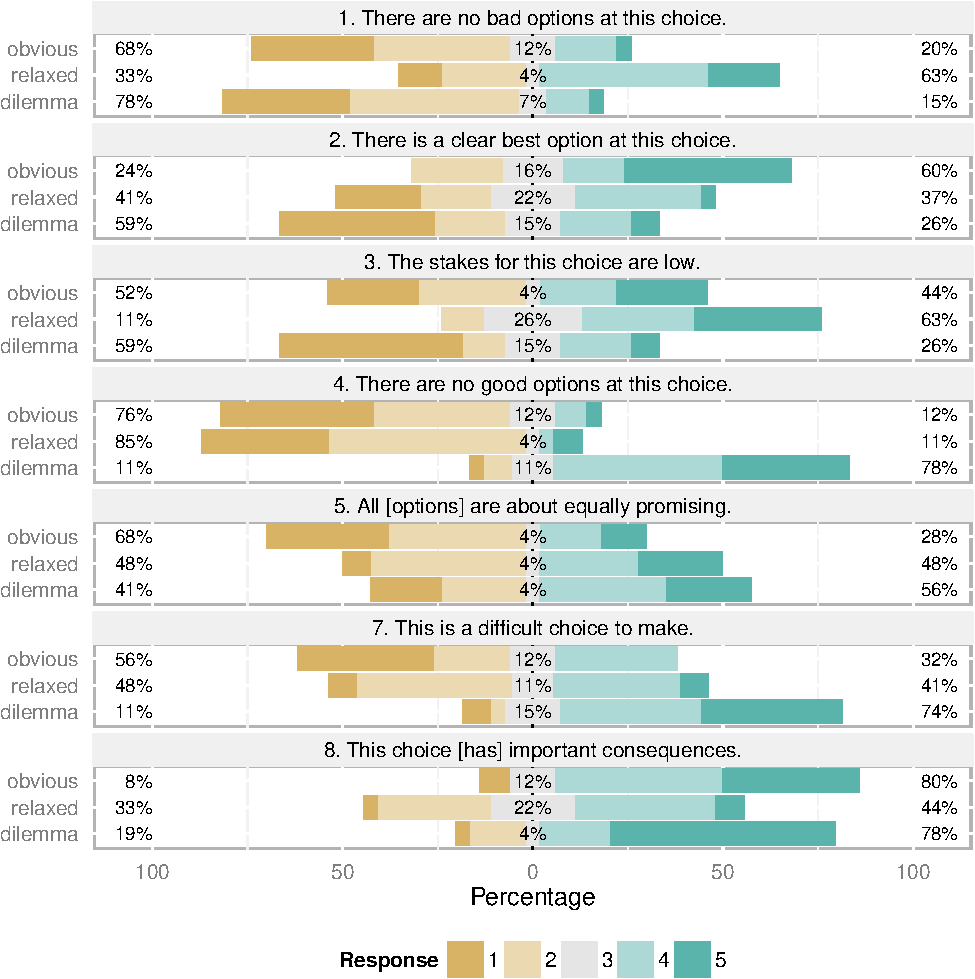
\includegraphics[height=0.85\textheight]{fig/combined-report-cropped.pdf}
\end{frame}

\begin{frame}{Results: Summary}
  \begin{itemize}\addtolength{\itemsep}{0.5\baselineskip}
    \item The question: \emph{``Is \dunyazad/ successfully creating the desired prospective impressions?''}
    \begin{itemize}\addtolength{\itemsep}{0.5\baselineskip}
      \vspace{0.5\baselineskip}
      \item In most ways, yes (20/25 hypotheses were confirmed).
      \item In some ways, no (it had trouble balancing options, creating choices without ``bad'' options, and creating easy choices).
    \end{itemize}
    \pause
    \item Can we figure out \emph{why} \dunyazad/ is failing?
    \pause
    \item $\rightarrow$ What are the lessons for choice poetics?
  \end{itemize}
\end{frame}

\begin{frame}{Lesson: Maximization and Satisfaction}
  \centering
  \includegraphics[width=\textwidth]{res/option-report-relaxed-nobad-detail.pdf} \\
  \raggedright
  \begin{itemize}\addtolength{\itemsep}{0.5\baselineskip}
    \item Relaxed choices have ``bad'' options?
    \item Maximizing vs\@. satisficing personalities. \\
      {\tiny \pcite{Schwartz2002}}
      \pause
    \item Some people identify ``worse'' options as ``bad'' options.
      \pause
    \item Context matters! Participants only saw a single choice.
    \item Balancing options will always be more difficult than contrasting them.
  \end{itemize}
\end{frame}

% TODO: Lesson: Relative Goal Priorities

\begin{frame}{Outline}
  \begin{itemize}
    \item Motivation
    \item Inspiration: \skald/ and \problemplanets/
    \item Methodology
    \item Related Work
    \item Theory: Choice Poetics
    \item Application: \dunyazad/
    \item Results: Options
    \item \textbf{Results: Outcomes}
    \item \textbf{Conclusions}
  \end{itemize}
\end{frame}

\begin{frame}{Outcomes Experiment}
  \begin{itemize}\addtolength{\itemsep}{0.5\baselineskip}
    \item Same setup as the first experiment, except participants made the choice and saw an outcome.
    \begin{itemize}\addtolength{\itemsep}{0.5\baselineskip}
      \vspace{0.5\baselineskip}
      \item 270 Amazon Mechanical Turk workers (+10 rejected).
      \item \$2.00 per task (one per worker).
      \item Median response time was 9:52.
      \item 205 valid responses (some duplicates due to an error).
      \item Five option questions (Likert) from the first study.
      \item Ten outcome questions (also 5-point Likert).
      \item Four multiple-choice motivation questions.
    \end{itemize}
  \end{itemize}
\end{frame}

\begin{frame}{Outcomes Experiment}
  \begin{itemize}\addtolength{\itemsep}{0.5\baselineskip}
    \item Three outcome variables: \textbf{valence}, \textbf{expectedness}, and \textbf{presence of viable alternatives}.
    \item Six experimental conditions: \\
      \vspace{0.5\baselineskip}
      \footnotesize
      \begin{tabular}{r c c c}
        \toprule
        & \textbf{Valence} & \textbf{Expectedness} & \textbf{Alternatives?} \\
        \midrule
        \textbf{Expected success} & good & expected & good \\
        \textbf{Expected failure} & bad & expected & bad \\
        \textbf{Unexpected failure} & bad & unexpected & good \\
        \textbf{Unexpected success} & good & unexpected & bad \\
        \textbf{Obvious Success}  & good & expected & bad \\
        \textbf{Obvious Faiure} & bad & unexpected & bad \\
        \bottomrule
      \end{tabular}
  \end{itemize}
\end{frame}

\begin{frame}{Survey Questions}
  \footnotesize
  \itshape
  \begin{enumerate}\addtolength{\itemsep}{0.5\baselineskip}
    \item ``Given the options available, the outcome I got is fair.''
    \item ``The outcome that I got makes sense given the option that I selected.''
    \item ``I got a bad outcome.''
    \item ``I'm happy with the option that I chose.''
    \item ``The outcome that I got is unfair, given the options available.''
    \item ``The outcome that I got is completely unexpected.''
    \item ``There is an outcome.'' ([This is a trick question])
    \item ``There might be a problem with this choice---the outcome I got does not make sense.''
    \item ``The outcome that I got is a good outcome.''
    \item ``I pretty much expected the outcome that I got.''
    \item ``I wish I had chosen a different option.''
  \end{enumerate}
\end{frame}

\begin{frame}{Survey Questions}
  \begin{itemize}\addtolength{\itemsep}{0.5\baselineskip}
    \item Five underlying concepts:
    \begin{enumerate}\addtolength{\itemsep}{0.5\baselineskip}
      \vspace{0.5\baselineskip}
      \item Fair vs\@. unfair.
      \item Sensible vs\@. incoherent.
      \item Good vs\@. bad.
      \item Satisfying vs\@. dissatisfying.
      \item Expected vs\@. unexpected.
    \end{enumerate}
  \end{itemize}
\end{frame}

%\begin{frame}{Results---Option Questions}
%  \centering
%  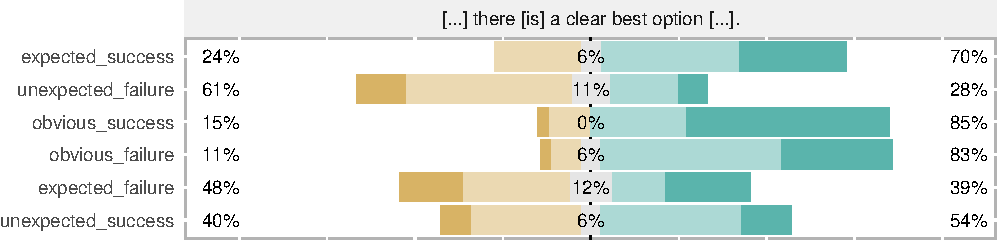
\includegraphics[width=0.8\textwidth]{{fig/cropped-outcomes-report-01-opt.obvious}.pdf} \\
%  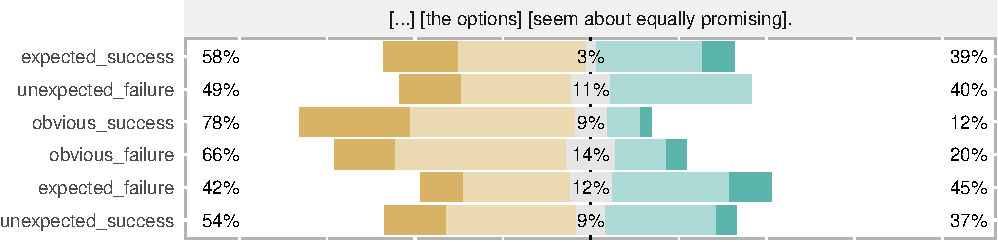
\includegraphics[width=0.8\textwidth]{{fig/cropped-outcomes-report-02-opt.balanced}.pdf} \\
%  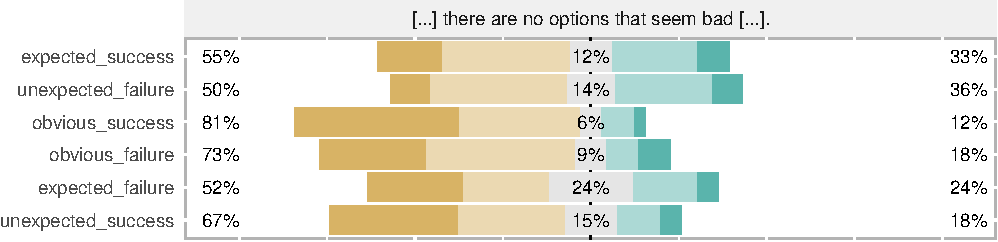
\includegraphics[width=0.8\textwidth]{{fig/cropped-outcomes-report-03-opt.nobad}.pdf} \\
%  
\includegraphics[width=0.8\textwidth]{fig/outcomes-legend-custom.pdf}
%\end{frame}
%
%\begin{frame}{Results---Option Questions}
%  \centering
%  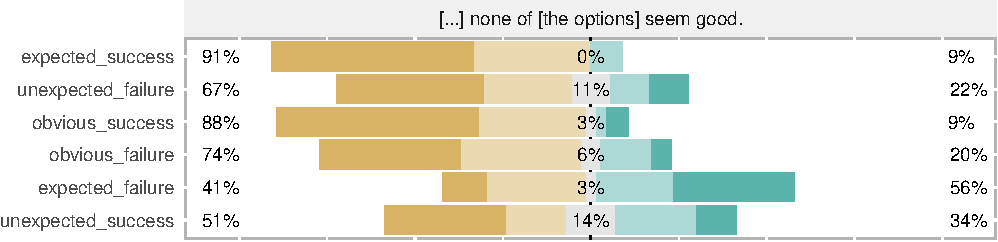
\includegraphics[width=0.8\textwidth]{{fig/cropped-outcomes-report-04-opt.nogood}.pdf} \\
%  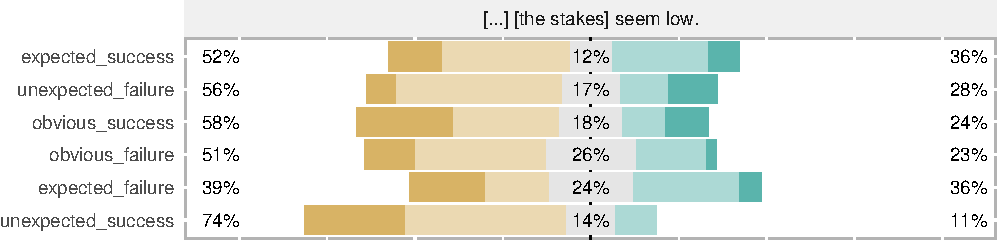
\includegraphics[width=0.8\textwidth]{{fig/cropped-outcomes-report-05-opt.stakes}.pdf} \\
%  
\includegraphics[width=0.8\textwidth]{fig/outcomes-legend-custom.pdf}
%\end{frame}
%
%
%\begin{frame}{Results---Fair/Unfair}
%  \centering
%  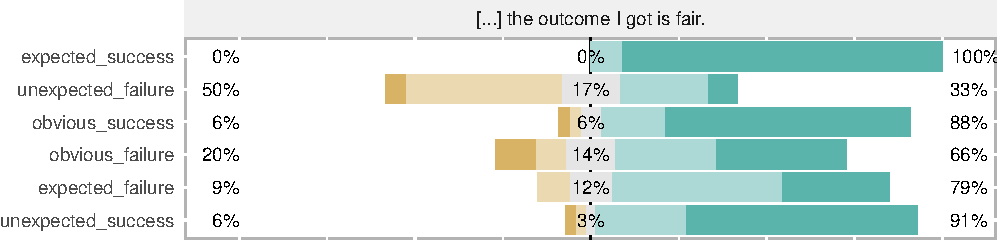
\includegraphics[width=\textwidth]{{fig/cropped-outcomes-report-10-out.fair}.pdf} \\
%  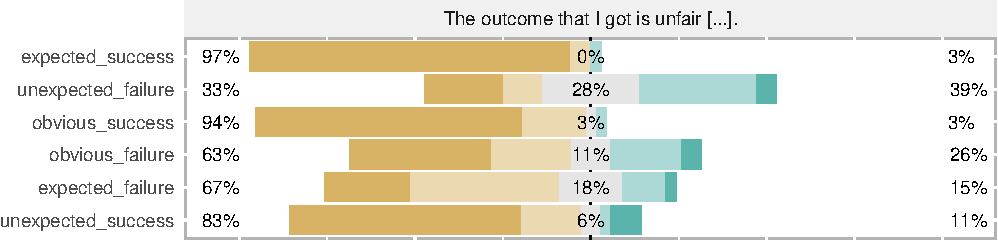
\includegraphics[width=\textwidth]{{fig/cropped-outcomes-report-11-out.unfair}.pdf} \\
%  
\includegraphics[width=\textwidth]{fig/outcomes-legend-custom.pdf}
%\end{frame}
%
%\begin{frame}{Results---Sense/Broken}
%  \centering
%  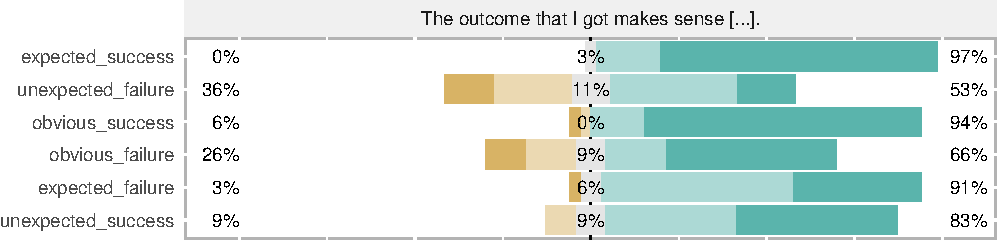
\includegraphics[width=\textwidth]{{fig/cropped-outcomes-report-12-out.sense}.pdf} \\
%  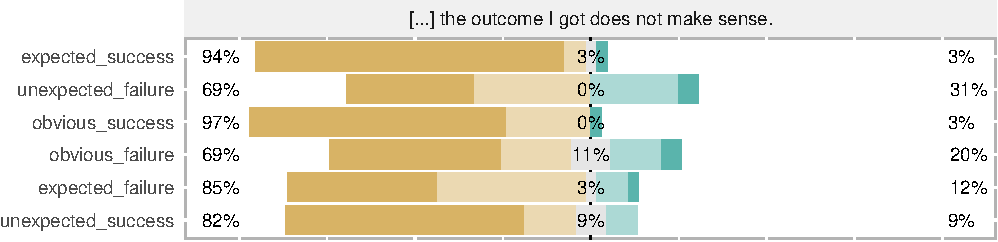
\includegraphics[width=\textwidth]{{fig/cropped-outcomes-report-13-out.broken}.pdf} \\
%  
\includegraphics[width=\textwidth]{fig/outcomes-legend-custom.pdf}
%\end{frame}

\begin{frame}{Results---Good/Bad}
  \centering
  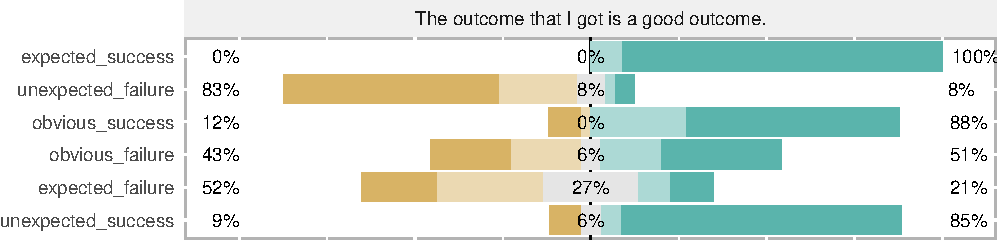
\includegraphics[width=\textwidth]{{fig/cropped-outcomes-report-06-out.good}.pdf} \\
  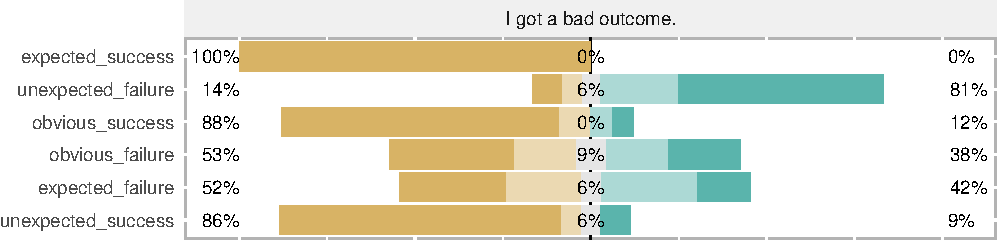
\includegraphics[width=\textwidth]{{fig/cropped-outcomes-report-07-out.bad}.pdf} \\
  
\includegraphics[width=\textwidth]{fig/outcomes-legend-custom.pdf}
\end{frame}

%\begin{frame}{Results---Satisfied/Dissatisfied}
%  \centering
%  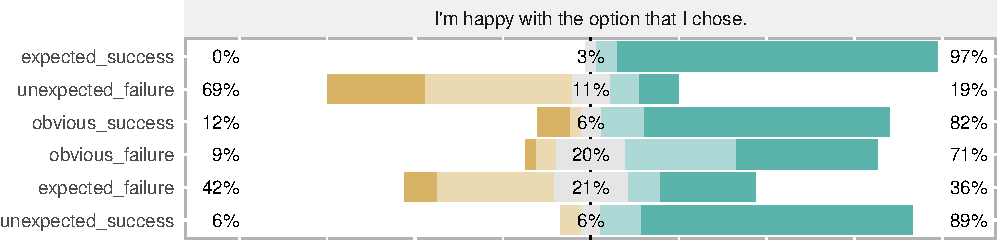
\includegraphics[width=\textwidth]{{fig/cropped-outcomes-report-14-out.happy}.pdf} \\
%  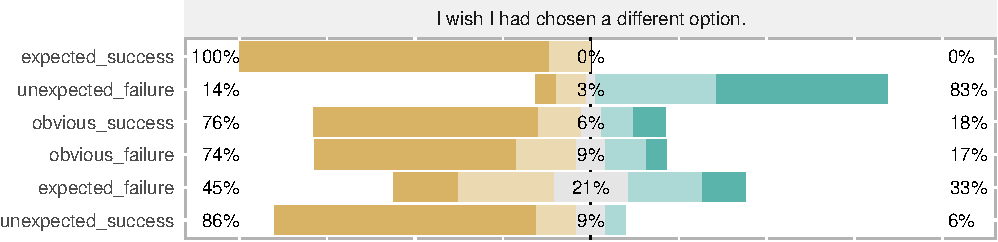
\includegraphics[width=\textwidth]{{fig/cropped-outcomes-report-15-out.regret}.pdf} \\
%  \includegraphics[width=\textwidth]{fig/outcomes-legend-custom.pdf}
%\end{frame}
%
%\begin{frame}{Results---Expected/Unexpected}
%  \centering
%  \includegraphics[width=\textwidth]{{fig/cropped-outcomes-report-08-out.expected}.pdf} \\
%  \includegraphics[width=\textwidth]{{fig/cropped-outcomes-report-09-out.unexpected}.pdf} \\
%  \includegraphics[width=\textwidth]{fig/outcomes-legend-custom.pdf}
%\end{frame}

\begin{frame}{Results: Summary}
  \begin{itemize}\addtolength{\itemsep}{0.5\baselineskip}
    \item The question: \emph{``Is \dunyazad/ successfully creating the desired retrospective impressions?''}
    \begin{itemize}\addtolength{\itemsep}{0.5\baselineskip}
      \vspace{0.5\baselineskip}
      \item For positive impressions, mostly (36/40 hypotheses confirmed).
      \item For negative impressions, only sometimes (17/36 hypotheses confirmed).
      \item There was trouble with surface text, moral reasoning, and weak expectations, among other things.
    \end{itemize}
    \item As before, \dunyazad/'s troubles offer plenty of feedback to the underlying theory.
  \end{itemize}
\end{frame}

\begin{frame}{Lesson: Impression Spillover}
  \centering
  {\sffamily Unexpected Success}
  \includegraphics[width=\textwidth]{{fig/cropped-detailed-report-unexpected\string_success-03-opt.nogood}.pdf} \\
  \includegraphics[width=\textwidth]{fig/detailed-outcomes-legend-custom.pdf}
  \raggedright
  \begin{itemize}\addtolength{\itemsep}{0.5\baselineskip}
    \item Choice 47794 seems to have at least one ``good'' option\ldots
    \pause
    \item Participants saw outcomes before judging options.
    \pause
    \item Choice 47794 was an \textbf{unexpected success} choice.
  \end{itemize}
\end{frame}

\begin{frame}{Choice 47794}
\scriptsize
\itshape
You come across some bandits attacking a merchant.
% 
The bandits are threatening the merchant.
% 
What do you do?

\begin{enumerate}
\item You talk the bandits down  \\
(You are missing skill: negotiation). \\[0.3em]
\item You transform the bandits into a chicken  \\
(You are missing skill: sorcery). \\[0.3em]
\item You attack the bandits  \\
(You are missing skill: fighting. They have skill: fighting. They have no tool for fighting). \\[0.3em]
\end{enumerate}
\end{frame}

\begin{frame}{Choice 47794}
\scriptsize
\itshape
You come across some bandits attacking a merchant.
% 
The bandits are threatening the merchant.
% 
What do you do?

\begin{enumerate}
\item You talk the bandits down  \\
(You are missing skill: negotiation). \\[0.3em]
\choicecount{6}$\rightarrow$ You reason with the bandits and the bandits agree to back off.  The bandits are no longer threatening the merchant. \\[-0.5em]
\item You transform the bandits into a chicken  \\
(You are missing skill: sorcery). \\[0.3em]
\choicecount{1}$\rightarrow$ You cast a spell on the bandits, and the bandits are cursed with the form of a chicken. The bandits are no longer threatening the merchant, they have been cursed and transformed into a chicken, and they are now not sentient. \\[-0.5em]
\item You attack the bandits  \\
(You are missing skill: fighting. They have skill: fighting. They have no tool for fighting). \\[0.3em]
\choicecount{3}$\rightarrow$ You attack them. They fight back but then they are hit by your attack and then you dodge the bandits' attack. They are defeated. You have acquired a book of herbal lore, the bandits are not threatening the merchant any more, and they have been killed.
\end{enumerate}
\end{frame}

\begin{frame}{Choice 47794}
\scriptsize
\itshape
You come across some bandits attacking a merchant.
% 
The bandits are threatening the merchant.
% 
What do you do?

\begin{enumerate}
\item You talk the bandits down  \\
  \textbf{(You are missing skill: negotiation)}. \\[0.3em]
\choicecount{6}$\rightarrow$ You reason with the bandits and the bandits agree to back off.  The bandits are no longer threatening the merchant. \\[-0.5em]
\item You transform the bandits into a chicken  \\
(You are missing skill: sorcery). \\[0.3em]
\choicecount{1}$\rightarrow$ You cast a spell on the bandits, and the bandits are cursed with the form of a chicken. The bandits are no longer threatening the merchant, they have been cursed and transformed into a chicken, and they are now not sentient. \\[-0.5em]
\item You attack the bandits  \\
(You are missing skill: fighting. They have skill: fighting. They have no tool for fighting). \\[0.3em]
\choicecount{3}$\rightarrow$ You attack them. They fight back but then they are hit by your attack and then you dodge the bandits' attack. They are defeated. You have acquired a book of herbal lore, the bandits are not threatening the merchant any more, and they have been killed.
\end{enumerate}
\end{frame}

\begin{frame}{Lesson: Impression Spillover}
  \begin{itemize}\addtolength{\itemsep}{0.5\baselineskip}
    \item Judgements of likelihood are influenced by results.
    \item Players learn as they play.
    \item A weak negative expectation can be revised into a neutral expectation.
    \item \emph{To create a success that seems surprising, strong negative expectations are required.}
  \end{itemize}
  \vfill
  \centering
  \tiny
  \pcite{Hall2012}
\end{frame}

% TODO: Motive results!

\begin{frame}{Outline}
  \begin{itemize}
    \item Motivation
    \item Inspiration: \skald/ and \problemplanets/
    \item Methodology
    \item Related Work
    \item Theory: Choice Poetics
    \item Application: \dunyazad/
    \item Results: Options
    \item Results: Outcomes
    \item \textbf{Conclusions}
  \end{itemize}
\end{frame}

\begin{frame}{\dunyazad/}
  \begin{itemize}\addtolength{\itemsep}{0.5\baselineskip}
    \item \dunyazad/ is moderately successful at creating choices with specific poetic properties, such as \textbf{obviousness} or \textbf{expectedness}.
    \item Explicit choice creation is a relatively novel generative domain.
    \item \dunyazad/ needs more work in order to generate full branching stories, and it has some holes that need patching.
  \end{itemize}
\end{frame}

\begin{frame}{Choice Poetics}
  \begin{itemize}\addtolength{\itemsep}{0.5\baselineskip}
    \item Choice poetics represents a recentering of several existing areas of research.
    \item My thesis foregrounds modes of engagement, discusses several poetic effects, and presents a novel analysis framework for analyzing choices based on player goals.
    \item The theory presented here allows for more specific and nuanced discussion of narrative choices.
    \item \dunyazad/'s successes show that goal-based choice analysis has \emph{generative} validity.
  \end{itemize}
\end{frame}

\begin{frame}{Experimental Humanities via AI}
  \begin{itemize}\addtolength{\itemsep}{0.5\baselineskip}
    \item Experimental results from \dunyazad/ have successfully been translated into specific caveats for the theory of choice poetics.
    \item Artificial intelligence enables \emph{experiment-driven} theory building in the humanities.
    \item In this case, the product of knowledge engineering is not just an AI system, but also \emph{new knowledge}.
  \end{itemize}
\end{frame}

\begin{frame}{Future Work}
  \begin{itemize}\addtolength{\itemsep}{0.5\baselineskip}
    \item Expand \dunyazad/ (in particular, add direct goal comparison).
    \item Revise choice poetics as appropriate and apply it to existing works.
    \item Look for more areas that could benefit from AI-enabled experimentation.
  \end{itemize}
\end{frame}

\begin{frame}{Questions?}
  \begin{itemize}
    \item Motivation
    \item Inspiration: \skald/ and \problemplanets/
    \item Methodology
    \item Related Work
    \item Theory: Choice Poetics
    \item Application: \dunyazad/
    \item Results: Options
    \item Results: Outcomes
    \item Conclusions
  \end{itemize}
\end{frame}

% MINSTREL Appendix:

\begin{frame}{\minstrel/}
  \justifying
  \setlength{\parindent}{1.5em}
  \itshape
  It was the spring of 1089, and a knight named Lancelot returned to Camelot from elsewhere. Lancelot was hot tempered. Once, Lancelot had lost a joust. Because he was hot tempered, Lancelot wanted to destroy his sword. Lancelot struck his sword. His sword was destroyed.

  One day, a lady of the court named Andrea wanted to have some berries\ldots
\end{frame}

\begin{frame}{\minstrel/}
  \vfill
  \begin{itemize}\addtolength{\itemsep}{0.5\baselineskip}
    \item Case-based story generation.
    \item Models human creativity through `Transform-Recall-Adapt Methods' (TRAMs).
    \item Manages story construction via `Author-Level Plans' (ALPs).
  \end{itemize}
  \vfill
  \centering
  \tiny
  \pcite{Turner1993}
\end{frame}

\begin{frame}{\skald/}
  \vfill
  \begin{itemize}\addtolength{\itemsep}{0.5\baselineskip}
    \item A rational reconstruction of \minstrel/.
    \item Focused on the TRAMs for imaginative recall.
    \item We experimented with different TRAM and ALP setups.
  \end{itemize}
  \vfill
  \centering
  \tiny
  \pcite{Tearse2014}
\end{frame}

\begin{frame}{\skald/: Experiments}
  \begin{itemize}\addtolength{\itemsep}{0.5\baselineskip}
    \item Results:
    \begin{itemize}\addtolength{\itemsep}{0.5\baselineskip}
      \vspace{0.5\baselineskip}
      \item TRAM configurations can trade coherence against variety.
      \item Modified boredom and TRAM selection can reduce search effort but also creativity.
    \end{itemize}
  \end{itemize}
  \vspace{1ex}
  \begin{tabular}{p{0.45\textwidth} p{0.45\textwidth}}
  \scriptsize
  \centering
  TRAM experiment: \newline
  \begin{tabular}{r c c}
      \toprule
      measure & orig. & mod. \\
      \midrule
      coherence & 35\% & 92\%  \\
      unique & 69 & 12 \\
      variation & 6.9 & 3.1  \\
      \bottomrule
  \end{tabular}
  &
  \scriptsize
  \centering
  Full system experiment: \newline
  \begin{tabular}{r c c}
      \toprule
      measure & orig. & mod. \\
      \midrule
      direct matches & 59\% & 72\% \\
      TRAMs tried & 13.8 & 7.7  \\
      TRAMs used & 2.4 & 1.4  \\
      \bottomrule
  \end{tabular} \newline
\end{tabular}
  \vfill
  \centering
  \tiny
  \pcite{Tearse2011} \\
  \pcite{Tearse2012}
\end{frame}

\begin{frame}{\problemplanets/}
  \begin{itemize}\addtolength{\itemsep}{0.5\baselineskip}
    \item A project to use \skald/ to build interactive vignettes.
    \item Vignettes would educate about climate change issues.
    \item The case library required delicate balancing.
    \item Coherence depended on complex ALPs.
    \item The placement of choices was static.
  \end{itemize}
\end{frame}

\begin{frame}{\problemplanets/}
  \begin{itemize}\addtolength{\itemsep}{0.5\baselineskip}
    \item Lessons:
    \begin{itemize}\addtolength{\itemsep}{0.5\baselineskip}
      \vspace{0.5\baselineskip}
      \item Focus on the consistency rules---raw material can be random.
      \item Come up with principles for placement and structure of choices.
    \end{itemize}
    \item $\rightarrow$ \dunyazad/
    \begin{itemize}\addtolength{\itemsep}{0.5\baselineskip}
      \vspace{0.5\baselineskip}
      \item A narrative generator focused on discrete choices.
      \item Uses answer-set programming to solve for story configurations.
    \end{itemize}
  \end{itemize}
\end{frame}

\end{document}
